% Written by: Erick Cobos T
% Date: 02-September-2016

\documentclass{beamer}

\usepackage{subcaption}
\usepackage{verbatim}


% To add sources at end
\newcommand{\source}[1]{\vskip0pt plus 1filll \scriptsize #1}

% Theme config
\usetheme{Madrid}
\usecolortheme{seahorse} %beaver for red, seahorse for blue


% Title information
\title[Progress Report]{Segmentation of Breast Cancer Masses in Digital Mammograms: A Convolutional Network}
\subtitle[Report]{Progress Report}
\author[Cobos] {Erick Cobos\inst{1}}
\date[September, 2016]{September, 2016}
\institute[Tec de Monterrey]{
	\inst{1} Centro de Sistemas Intelligentes \\ Tecnologico de Monterrey
}
%\subject{Subject}



\begin{document}

	\begin{frame}
		\titlepage
		% the objective of this talk is to report the progress of my thesis, explain what I have been doing it, why I choose to do what I'm doing, what i'm still left to do and receive feedback from the commitee.
	\end{frame}
		
	% Table of contents
	\begin{frame}
		\frametitle{Table of Contents}
		\tableofcontents[currentsection]
    \end{frame}
    
    \section[Introduction]{Introduction}
    \begin{frame}
		\frametitle{Thesis objective}
			The main goal is to segment breast cancer lesions using convolutional networks, an end-to-end learnable model.
		
		\begin{itemize}
			\item Obtain and process the mammographic database. %to make it available for future research on campus.
			\item Develop software to handle the database and train new deep learning models.
			\item Train modern, fine-tuned convolutional networks.% to perform lesion segmentation.
			\item Test the viability of convolutional networks for breast cancer research.
			\item Propose ideas for future research in the area.
		\end{itemize}
	\end{frame}

    \section[Lesion Segmentation]{Lesion Segmentation}
    \begin{frame}
     	\frametitle{Why breast cancer}
     		Breast cancer is the most commonly diagnosed cancer among women.
     		
     		For women, death rates are the second highest of any cancer. However, survival rate when detected early is close to 100\%.
     		
     		On-going project at the institution.
    \end{frame}
%Cancer es un término que se usa para describir varias enfermedades distintas donde celulas anomalas se dividen sin control produciendo tuimores y eventualmente invadiendo tejido cercano. Breast cancer es cuando se genera en tejidos del seno.
%Besides skin cancer, breast cancer is one of the most commonly diagnosed cancer among American women.  Just under 30% of cancers in women are breast cancers. 
%About 1 in 8 U.S., UK women will develop invasive breast cancer.
%Death rates higher than those for any other cancer, besides lung cancer.
%People in the campus have been wporking on this already.

    
	\begin{frame}
		\frametitle{Breast cancer signs}
		Masses vs. microcalcifications
		\begin{figure}[h]
			\centering
			\begin{subfigure}{0.35\textwidth}
				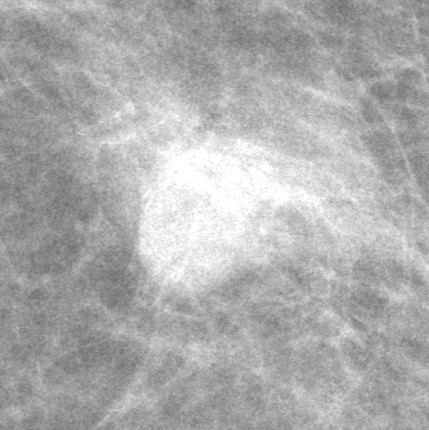
\includegraphics[width=\textwidth]{plots/breastMass.jpg}
			\end{subfigure}
			~
			\begin{subfigure}{0.35\textwidth}
				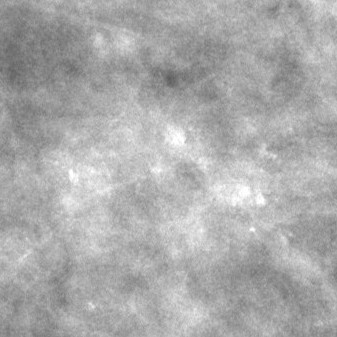
\includegraphics[width=\textwidth]{plots/breastMicrocalcification.jpg}
			\end{subfigure}
		\end{figure}

		Detection vs. diagnosis
	\end{frame}
% Mammography is the main tool. we focus on this and this.
	
	\begin{frame}
		\frametitle{Lesion segmentation}
		\begin{figure}[h]
			\centering
			\begin{subfigure}{0.35\textwidth}
				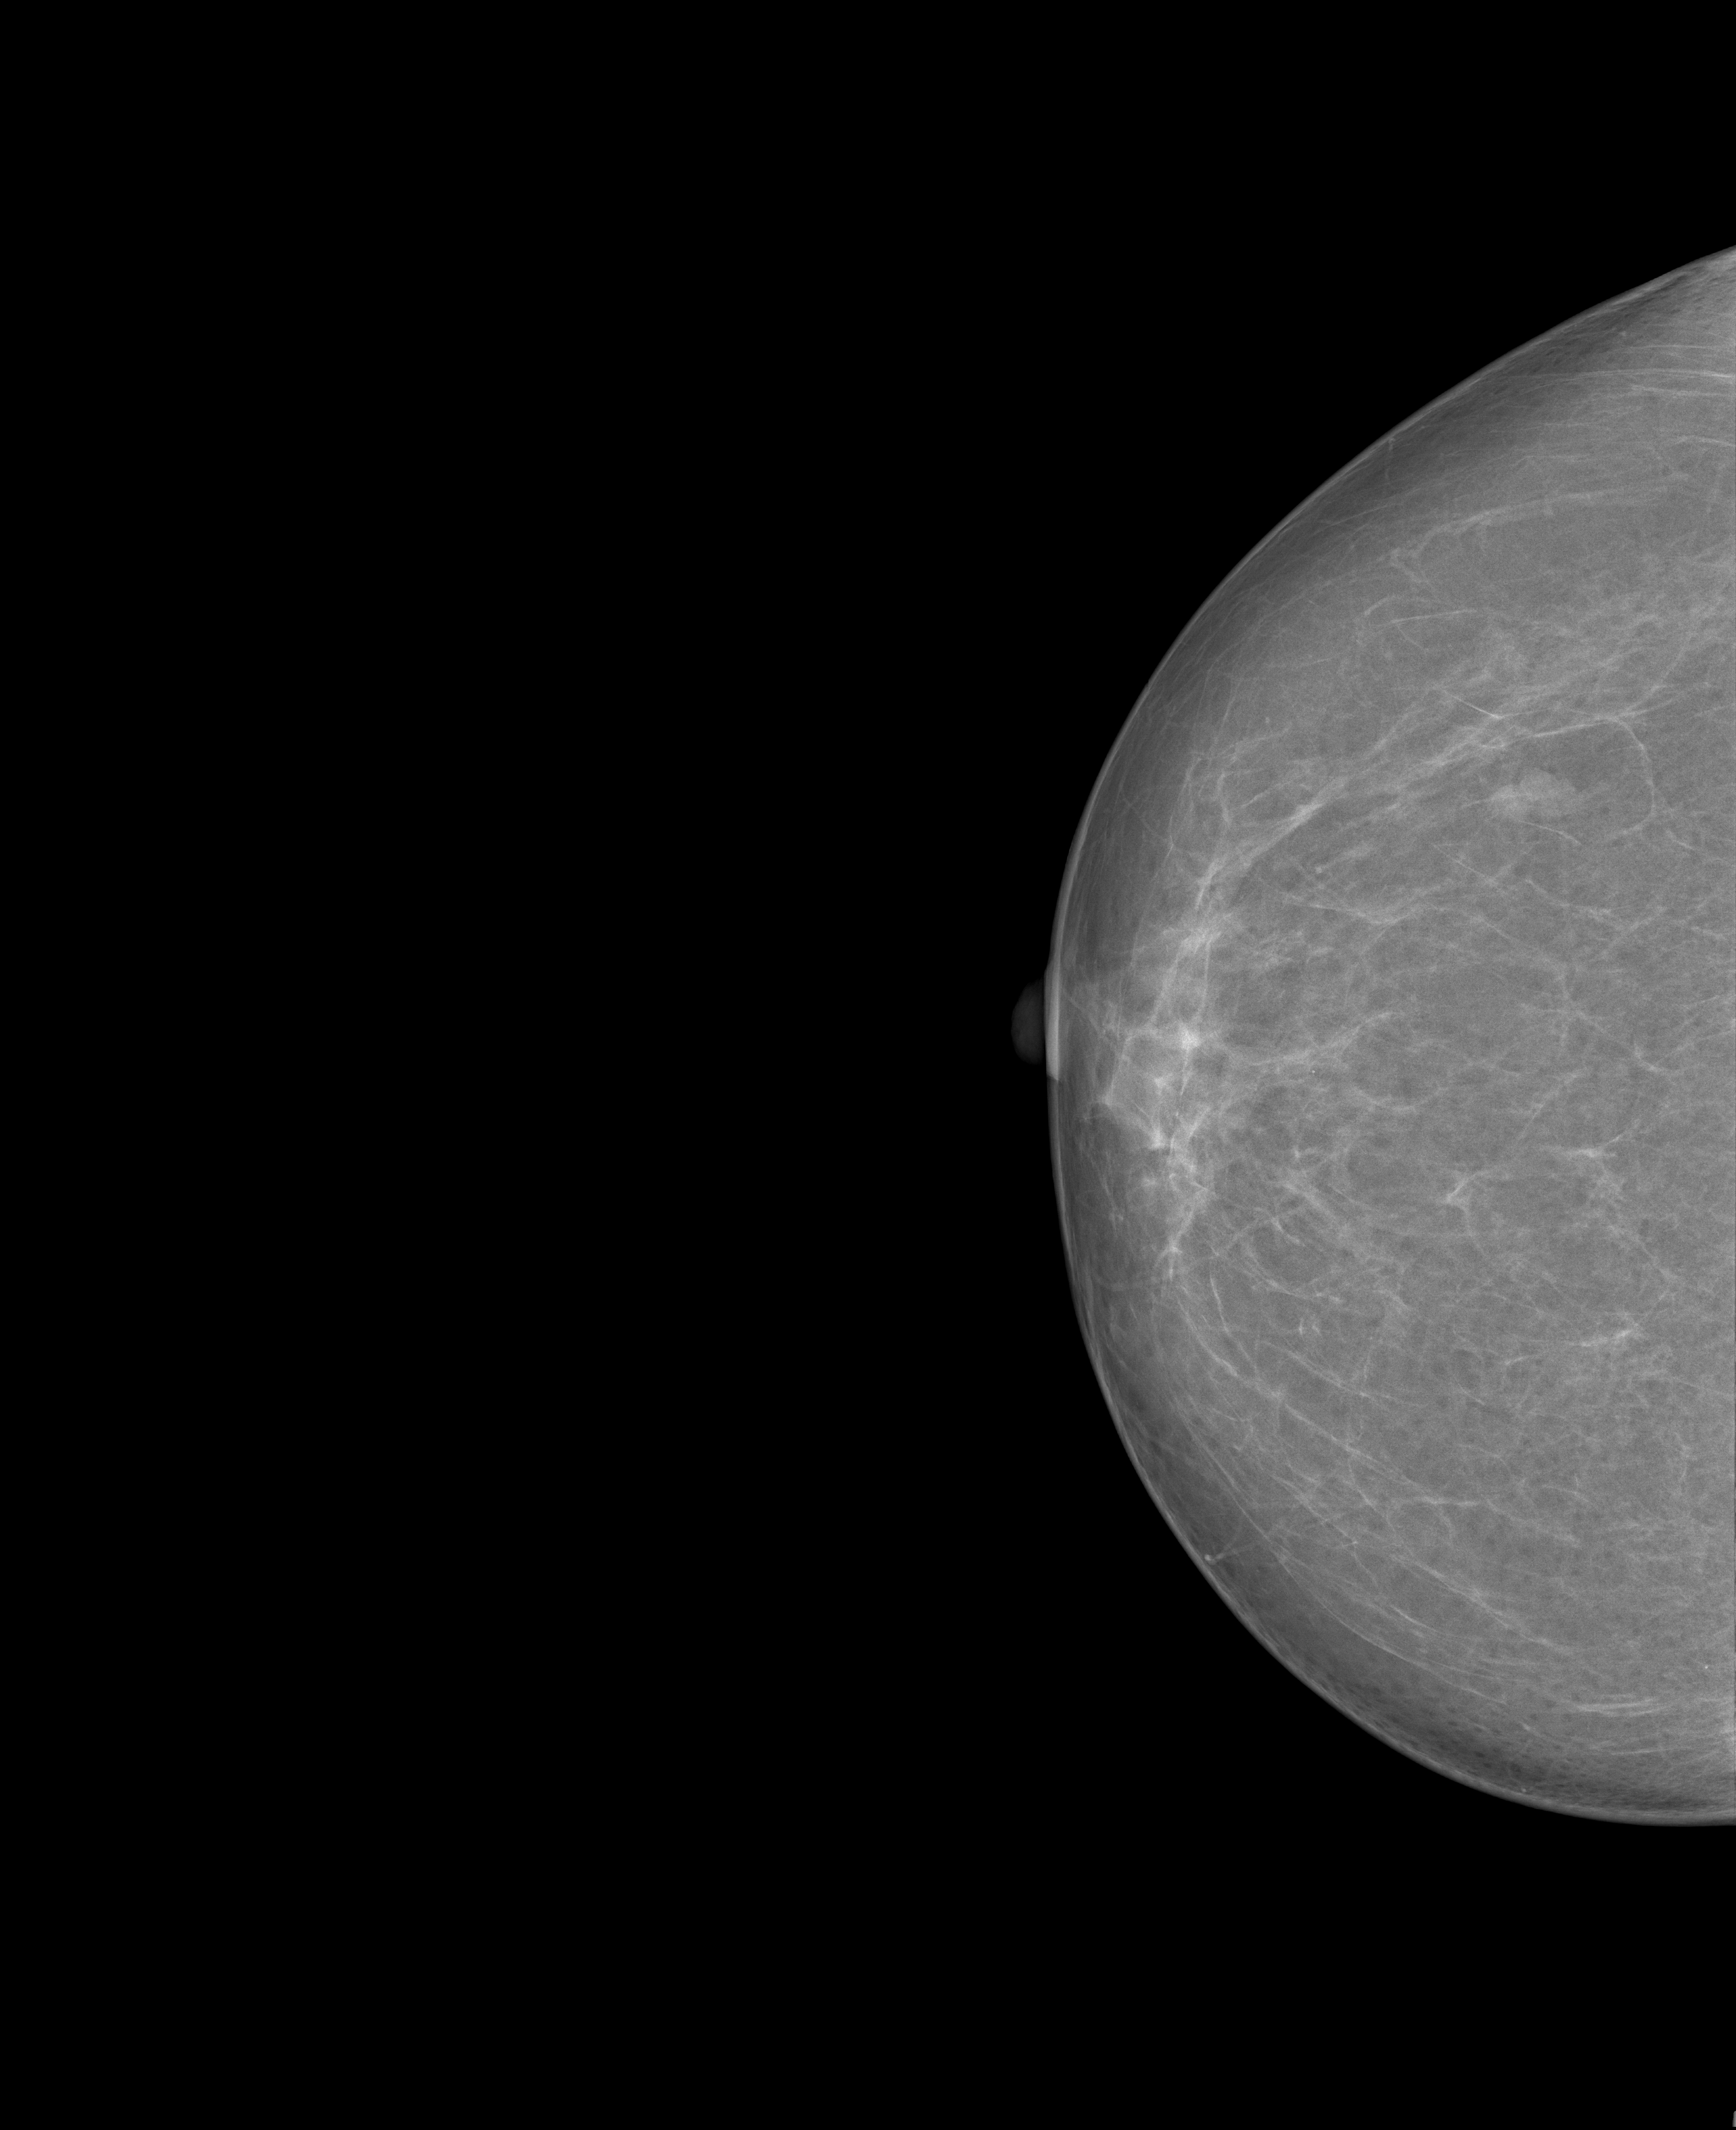
\includegraphics[width=\textwidth]{plots/mammogram.png}
				\caption{Mammogram}
			\end{subfigure}
			~
			\begin{subfigure}{0.35\textwidth}
				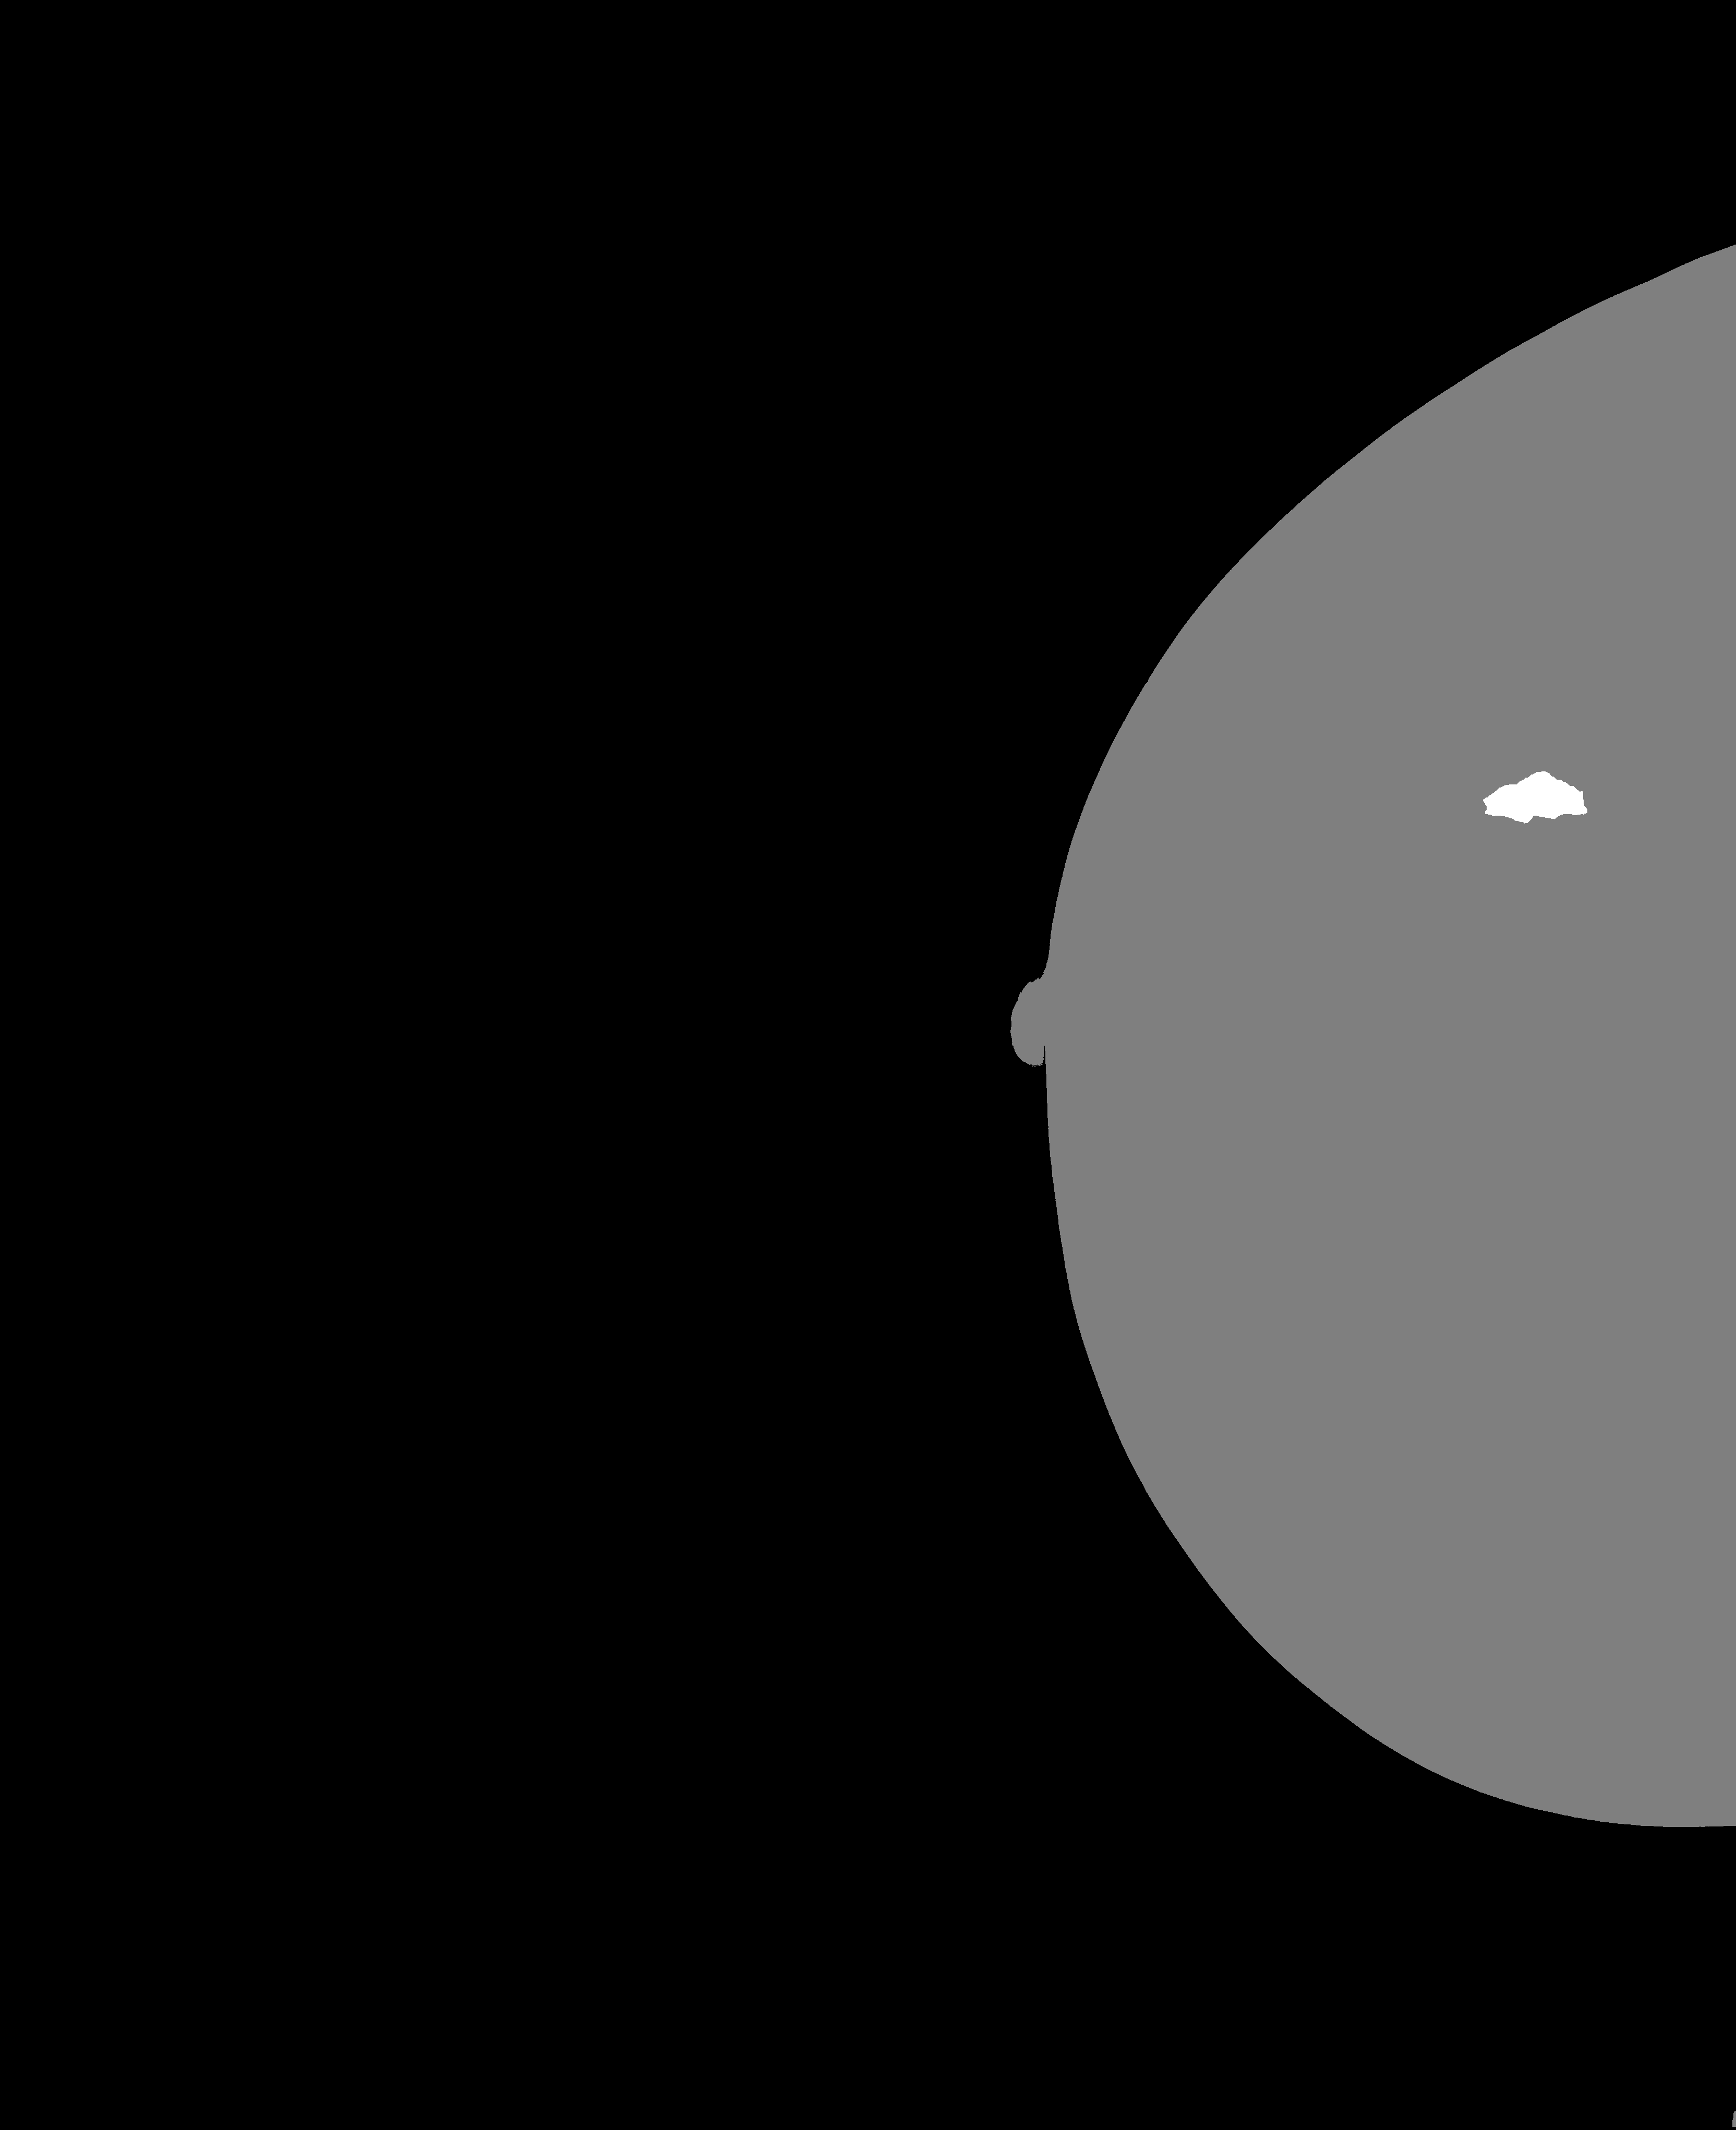
\includegraphics[width=\textwidth]{plots/label.png}
				\caption{Segmentation}
			\end{subfigure}
		% img_108_146_1_RCC.png
		\end{figure}
	\end{frame}
	
	
	\section[Convolutional networks]{Convolutional networks}
	\begin{frame}
	\frametitle{Why convolutional networks?}
		\begin{itemize}
			\item Convnets have showed great results in image classification tasks.
			\item Convnets learn which features are important for the classification. 
	 		\item We don’t need experts to carefully handcraft and select features.
		\end{itemize}
		\vfill
		Cons: Need processing power, data.
	\end{frame}
% From 2012 to now they have been used everywhere become standard in image processing, if there is a breakthrough in computer vision, most probably is donde with convnets.
% ImageNet (super-human ability) They can be used as is for image segmentation.
% Everything is learned, end-to-end

	\subsection[Classification]{Classification}
	\begin{frame}
		\frametitle{Convolutional networks}
		Learnable filters: spatially local and simple in early layers, global and complex in deeper layers.
		\begin{figure}[h]
			\centering
			\begin{subfigure}{0.4\textwidth}
				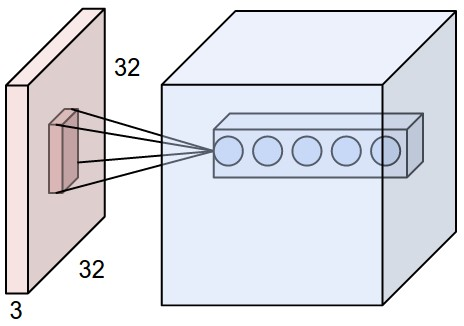
\includegraphics[width=\textwidth]{plots/convLayer.jpeg}
			\end{subfigure}
			~
			\begin{subfigure}{0.5\textwidth}
				\begin{subfigure}{\textwidth}
					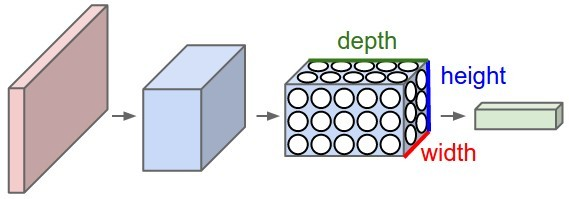
\includegraphics[width=\textwidth]{plots/convNetVolumes.jpeg}
				\end{subfigure}
				\par \smallskip
				\begin{subfigure}{\textwidth}
					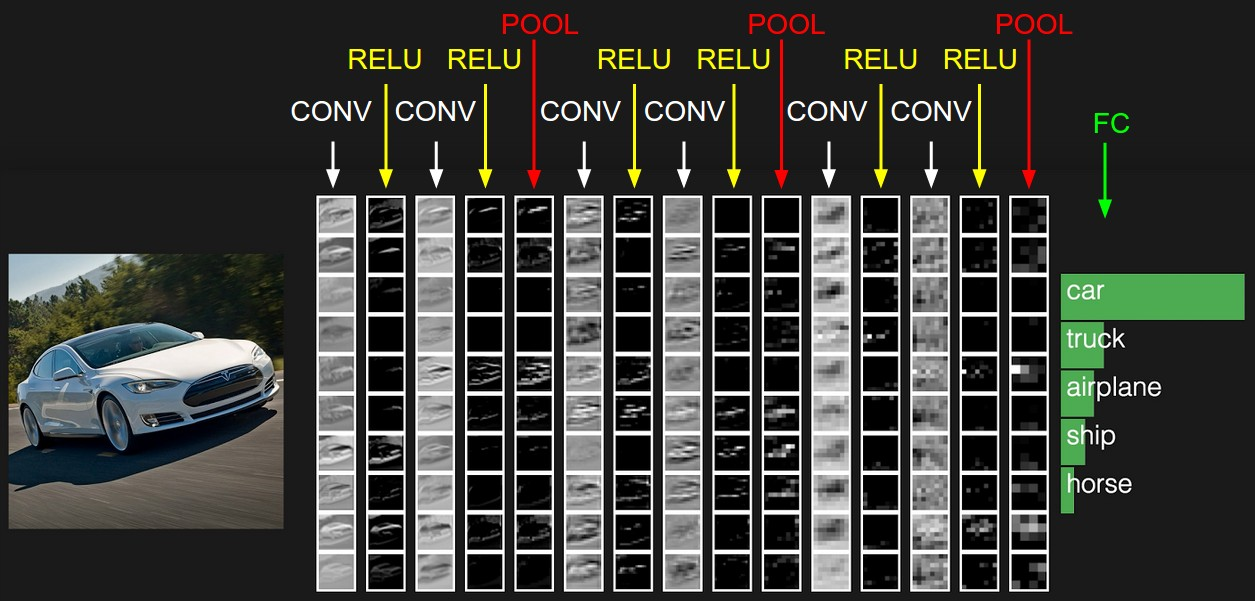
\includegraphics[width=\textwidth]{plots/convNetExample.jpeg}
				\end{subfigure}
			\end{subfigure}
		\end{figure}
		\source{[Karpathy et al., 2016]}
		% Explain kernels and hierarchichal features
	\end{frame}
		
	\begin{frame}
		\frametitle{What have they done}
		\vspace{30pt}
		\begin{figure}[h]
			\centering
			\begin{subfigure}{\textwidth}
				
\includegraphics[width=\textwidth]{plots/imageNetLogo.png}
			\end{subfigure}
			\par\smallskip
			\begin{subfigure}{0.35\textwidth}
				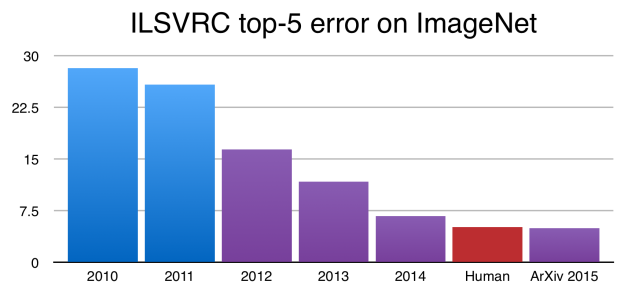
\includegraphics[width=\textwidth]{plots/imageNetAdvances.png}
			\end{subfigure}
			~
			\begin{subfigure}{0.6\textwidth}
				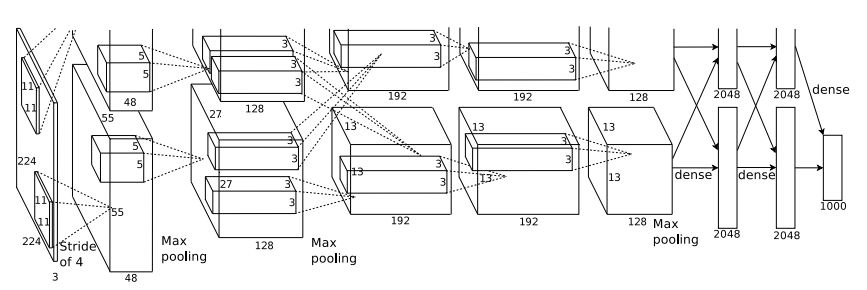
\includegraphics[width=\textwidth]{plots/alexnet.png}
			\end{subfigure}
		\end{figure}
		\source{[Nvidia Corp., 2015], [Krizhevsky et al., 2012]}
		% Explain ImageNet and talk about results
	\end{frame}
	
	\begin{frame}
		\frametitle{Architectures}
		\begin{figure}[h]
			\centering
			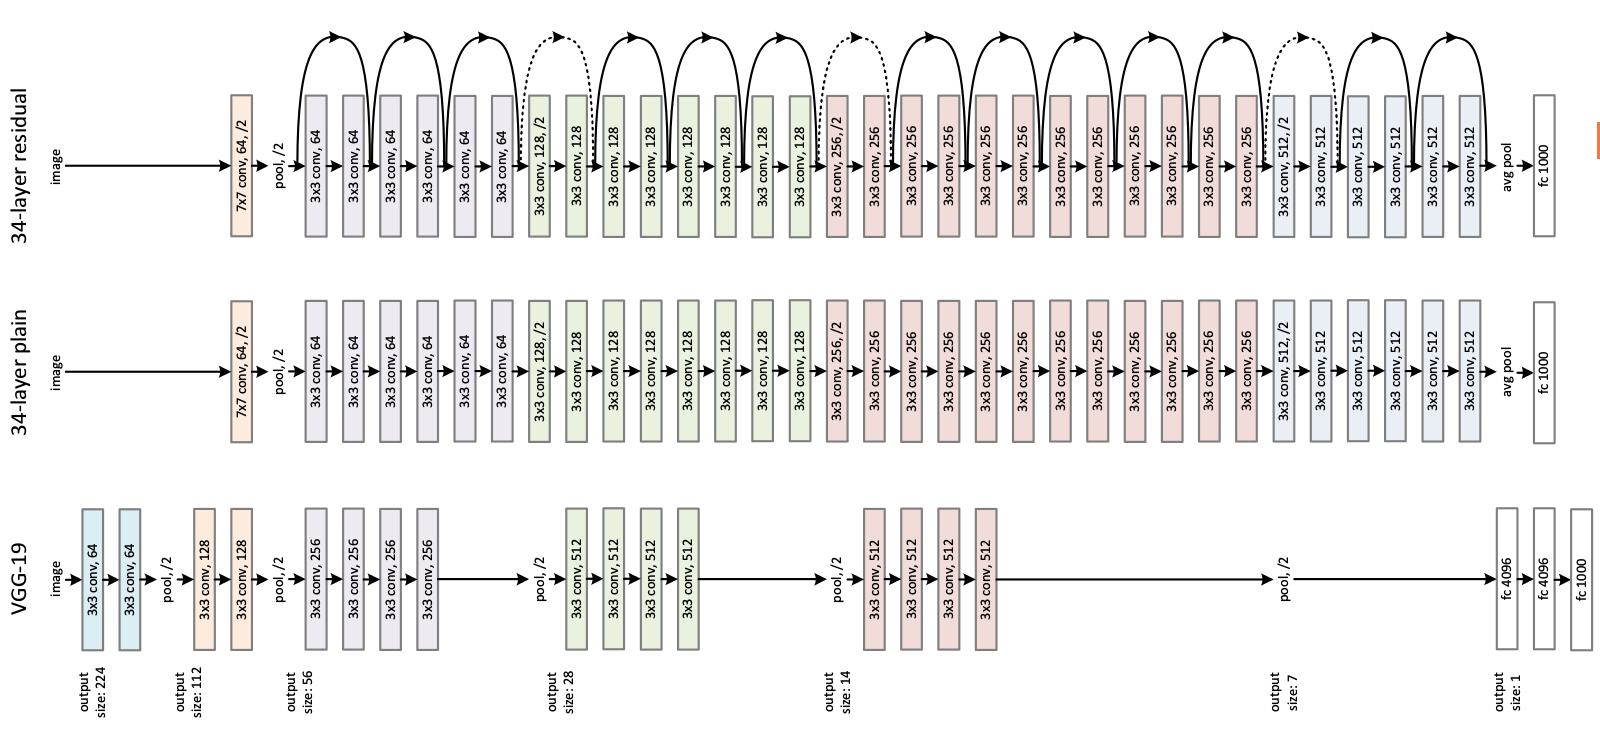
\includegraphics[width=\textwidth]{plots/resNet.png}
		\end{figure}
		
		Deeper, no pooling layers, no fully-connected layers, no dropout, all 3x3 kernels, batch normalization, residual connections, attention, memory...
		\source{[He et al., 2015]}
		% VGG-net and ResNet-like/other things
		% Deeper, no pooling, no fc, no dropout, batchnorm, residual connections
		% all 3x3 convolutions
	\end{frame}

	\subsection[Segmentation]{Segmentation}
	\begin{frame}
		\frametitle{Segmentation}
		Solved by upsampling, deconvolution or dilated convolutions.
		\begin{figure}[h]
			\centering
			\begin{subfigure}{0.45\textwidth}
				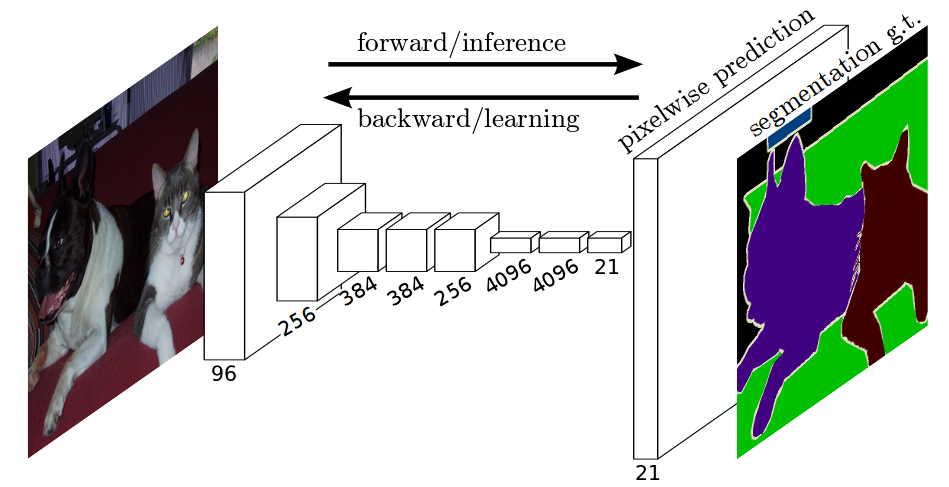
\includegraphics[width=\textwidth]{plots/fcn.png}
			\end{subfigure}
			~
			\begin{subfigure}{0.5\textwidth}
				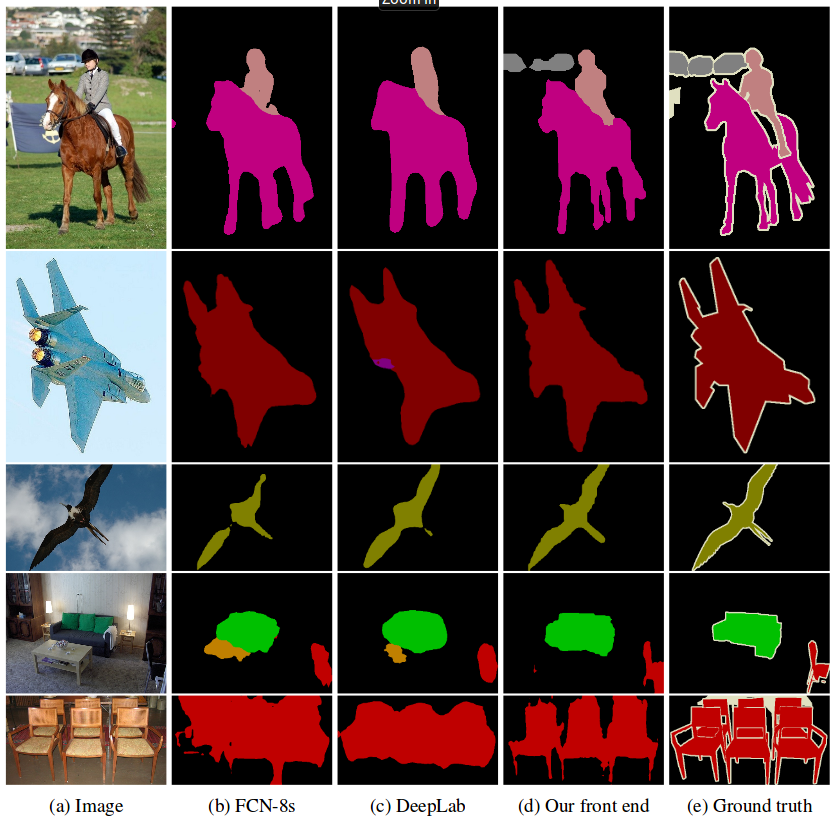
\includegraphics[width=\textwidth]{plots/segmentationComparison.png}
			\end{subfigure}
		\end{figure}
		\source{[Longet al., 2015], [Yu and Koltun, 2016]}
		% Explain how kernels are moved along to produce a full result
	\end{frame}
	% Traditional way. Image visión, specialized techniques. Handcrafted features made by experts But it is hard to design this, and it takes time to maintain, and you need expertise: end-to-end, learn from data, not done by hand. Pipeline
	% Completely automatic, single step v. pipeline.


	\section[Work done]{Work done}
	\begin{frame}
		\frametitle{Literature review}
		\vspace{15pt}
		\begin{figure}[h]
			\centering
			\begin{subfigure}{0.48\textwidth}
				\begin{subfigure}{\textwidth}
					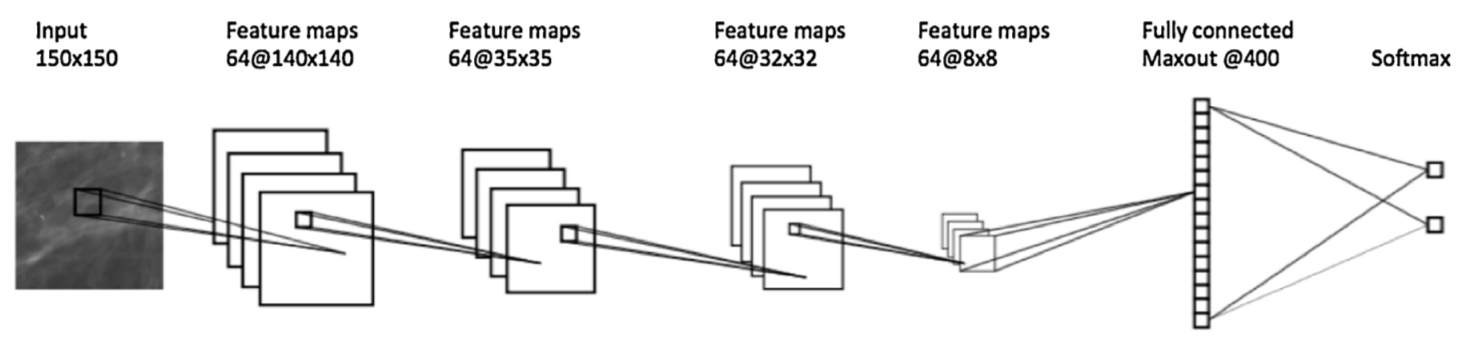
\includegraphics[width=\textwidth]{plots/arevalo.png}
				\end{subfigure}
				~
				\begin{subfigure}{\textwidth}
					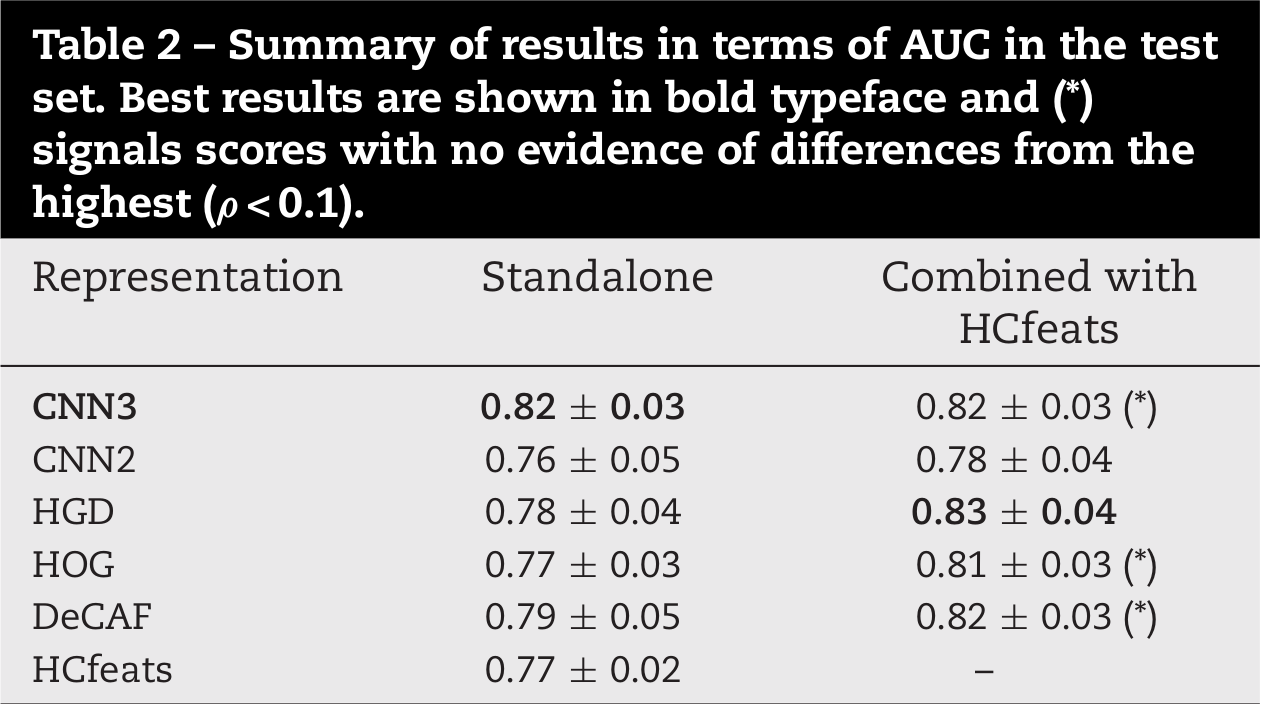
\includegraphics[width=\textwidth]{plots/arevaloResults.png}
				\end{subfigure}
				\caption{Mass diagnosis (4 layers, 3.4M params)}
			\end{subfigure}
			~
			\begin{subfigure}{0.48\textwidth}
				\begin{subfigure}{\textwidth}
					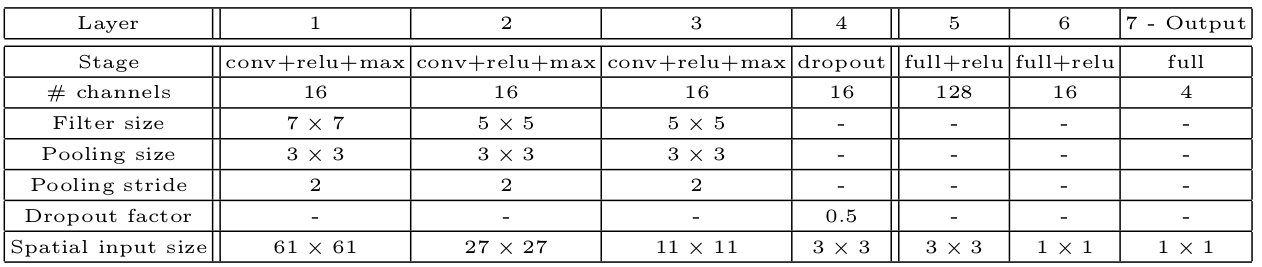
\includegraphics[width=\textwidth]{plots/dubrovina1.png}
				\end{subfigure}
				~
				\begin{subfigure}{\textwidth}
					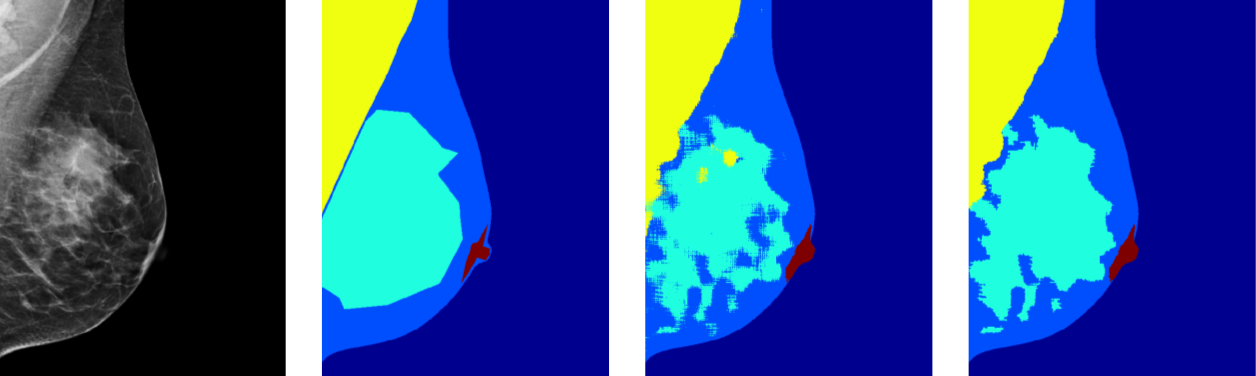
\includegraphics[width=\textwidth]{plots/dubrovina2.png}
				\end{subfigure}
				~
				\begin{subfigure}{\textwidth}
					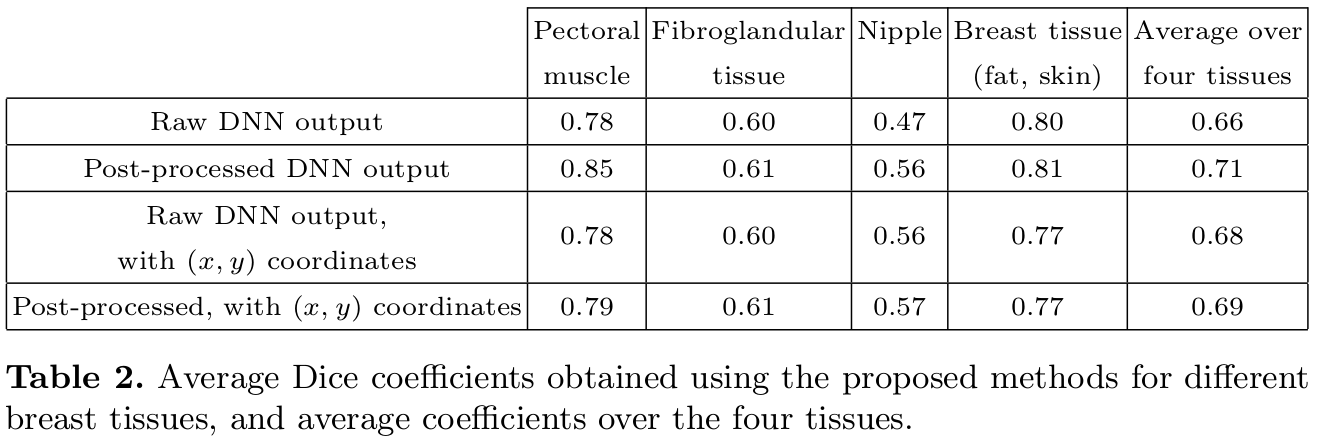
\includegraphics[width=\textwidth]{plots/dubrovinaResults.png}
				\end{subfigure}
				\caption{Tissue segmentation (6 layers, 34K params)}
			\end{subfigure}
		\end{figure}
		\source{[Arevalo et al., 2016], [Dubrovina et al.,2015]}
		% What has been done in breast cancer, Wrote background, examples and accuracies
	\end{frame}
	
	\begin{frame}
		\frametitle{Database preprocessing}
		\begin{figure}[h]
		\centering
			\begin{subfigure}{0.24\textwidth}
				\centering
					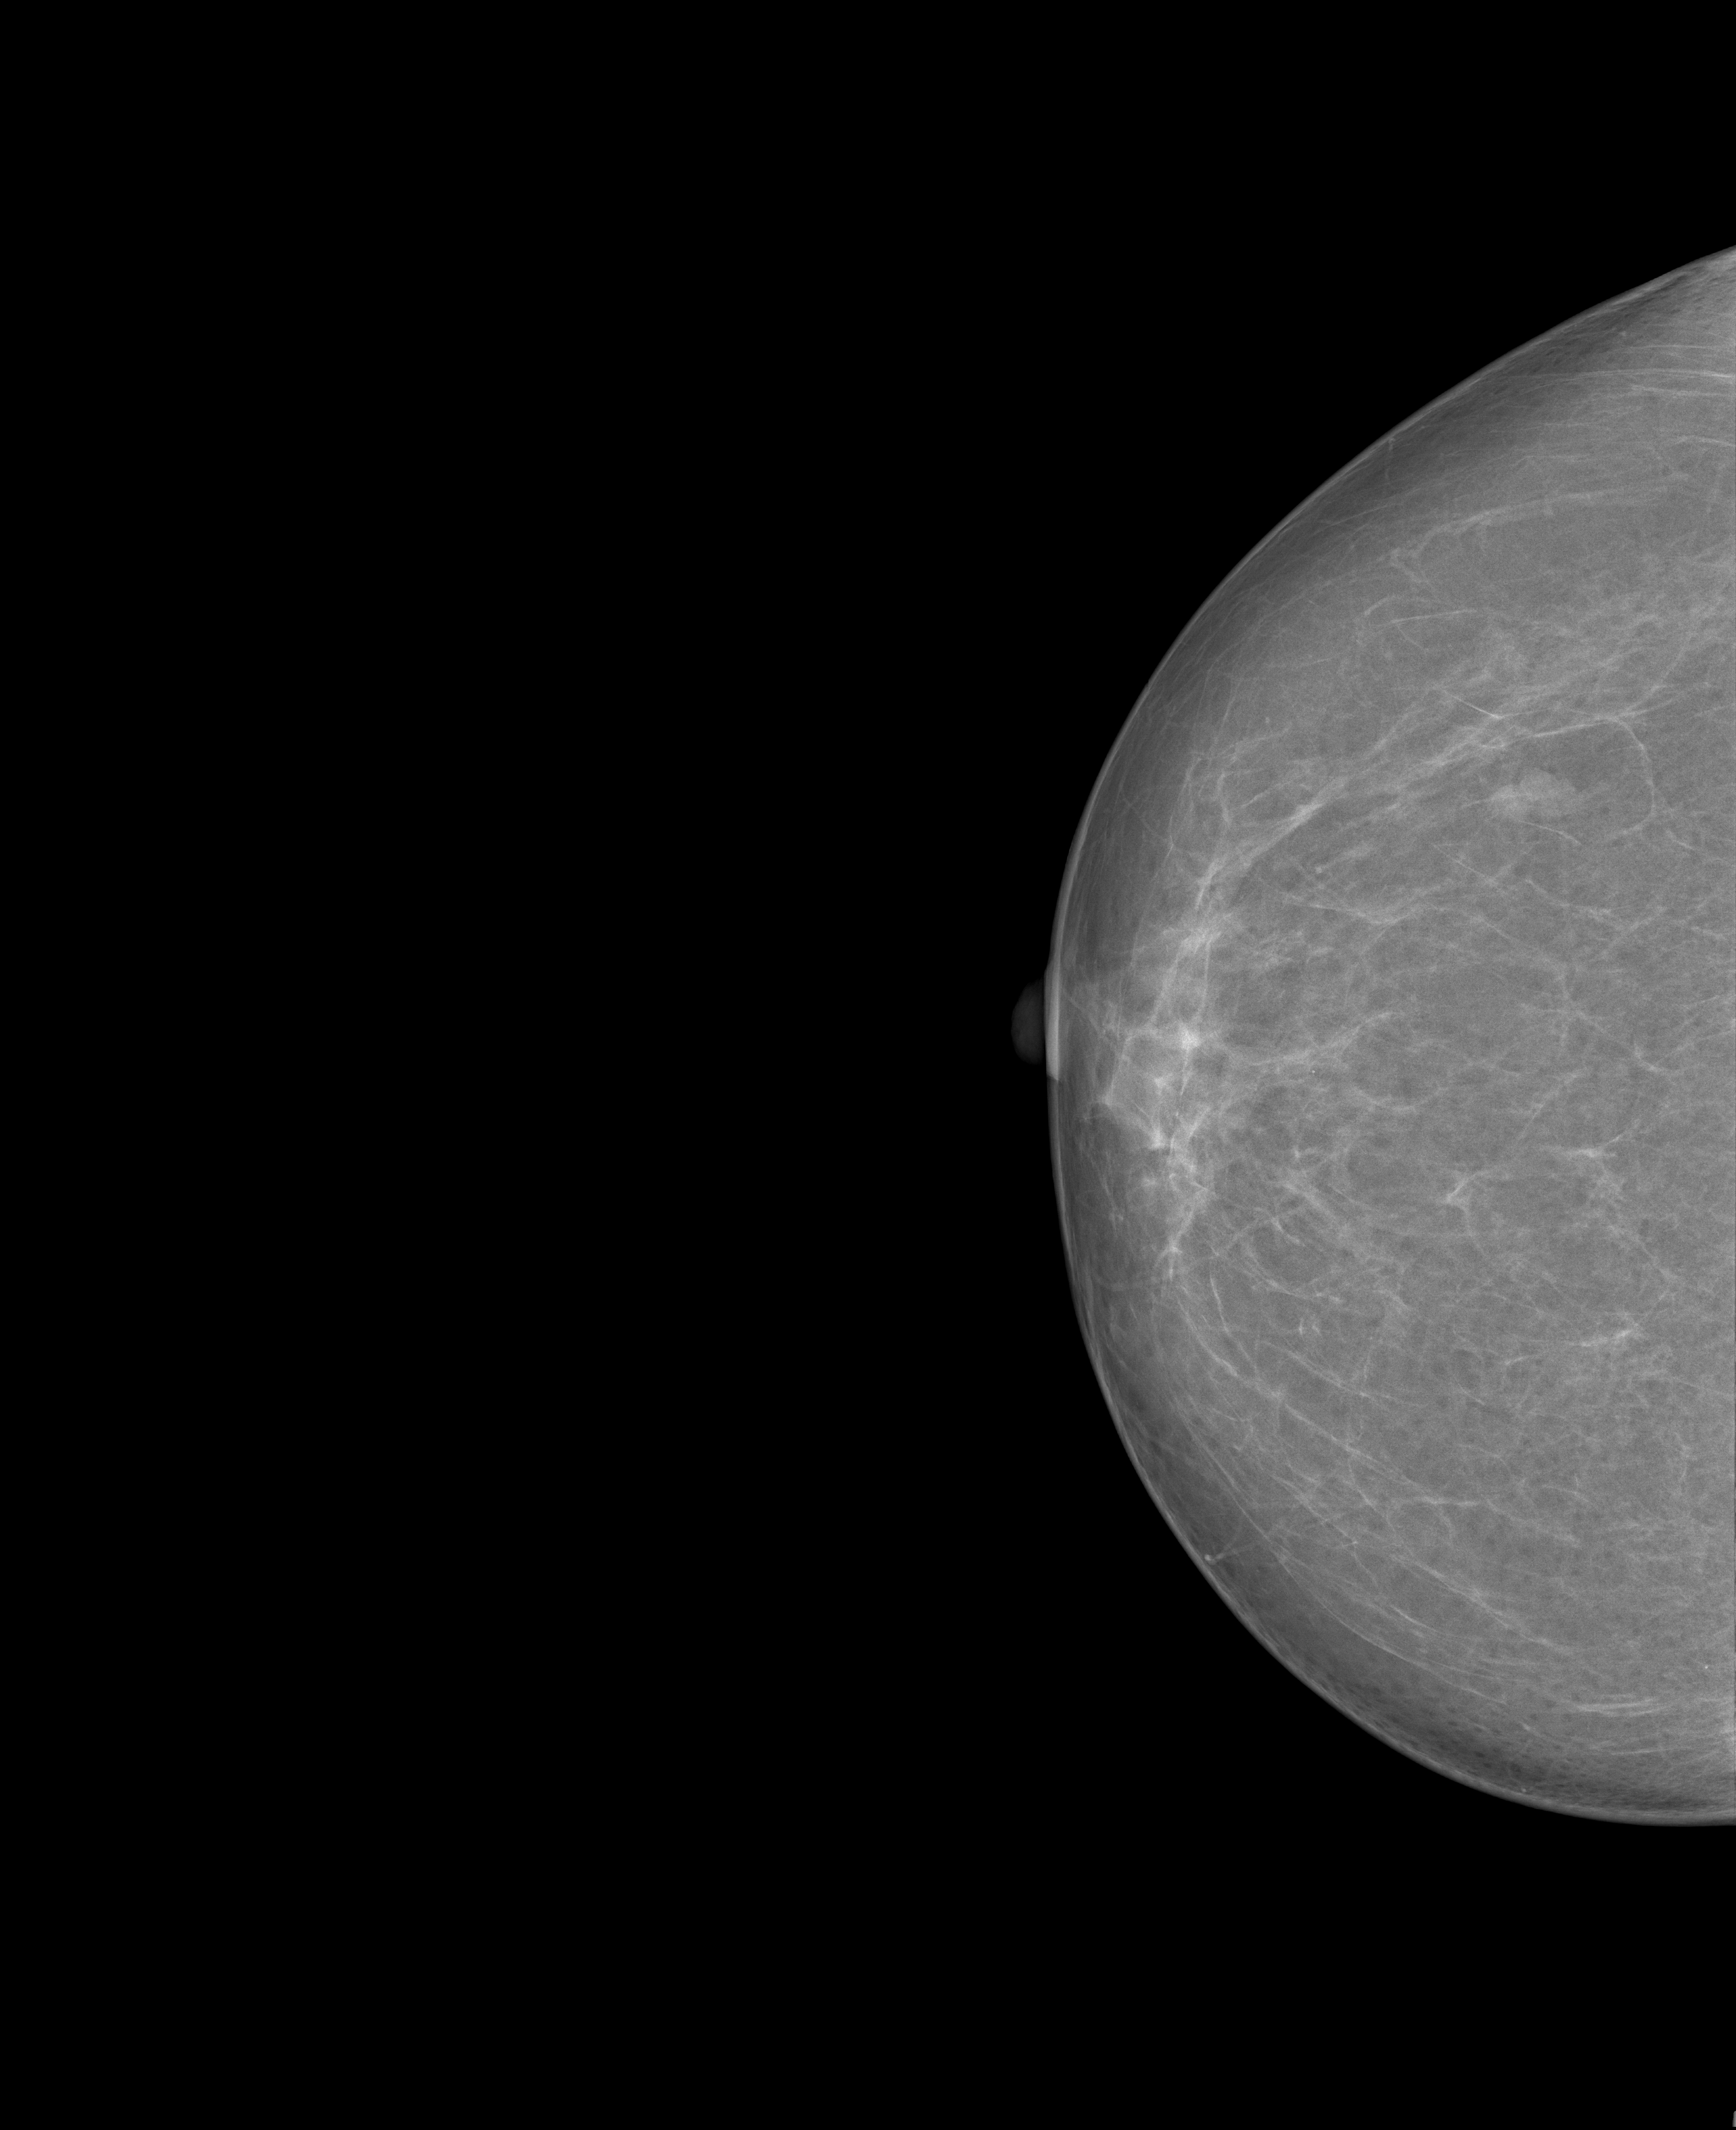
\includegraphics[height=3.5cm]{plots/mammogram.png}
			\end{subfigure}
			\begin{subfigure}{0.24\textwidth}
				\centering
					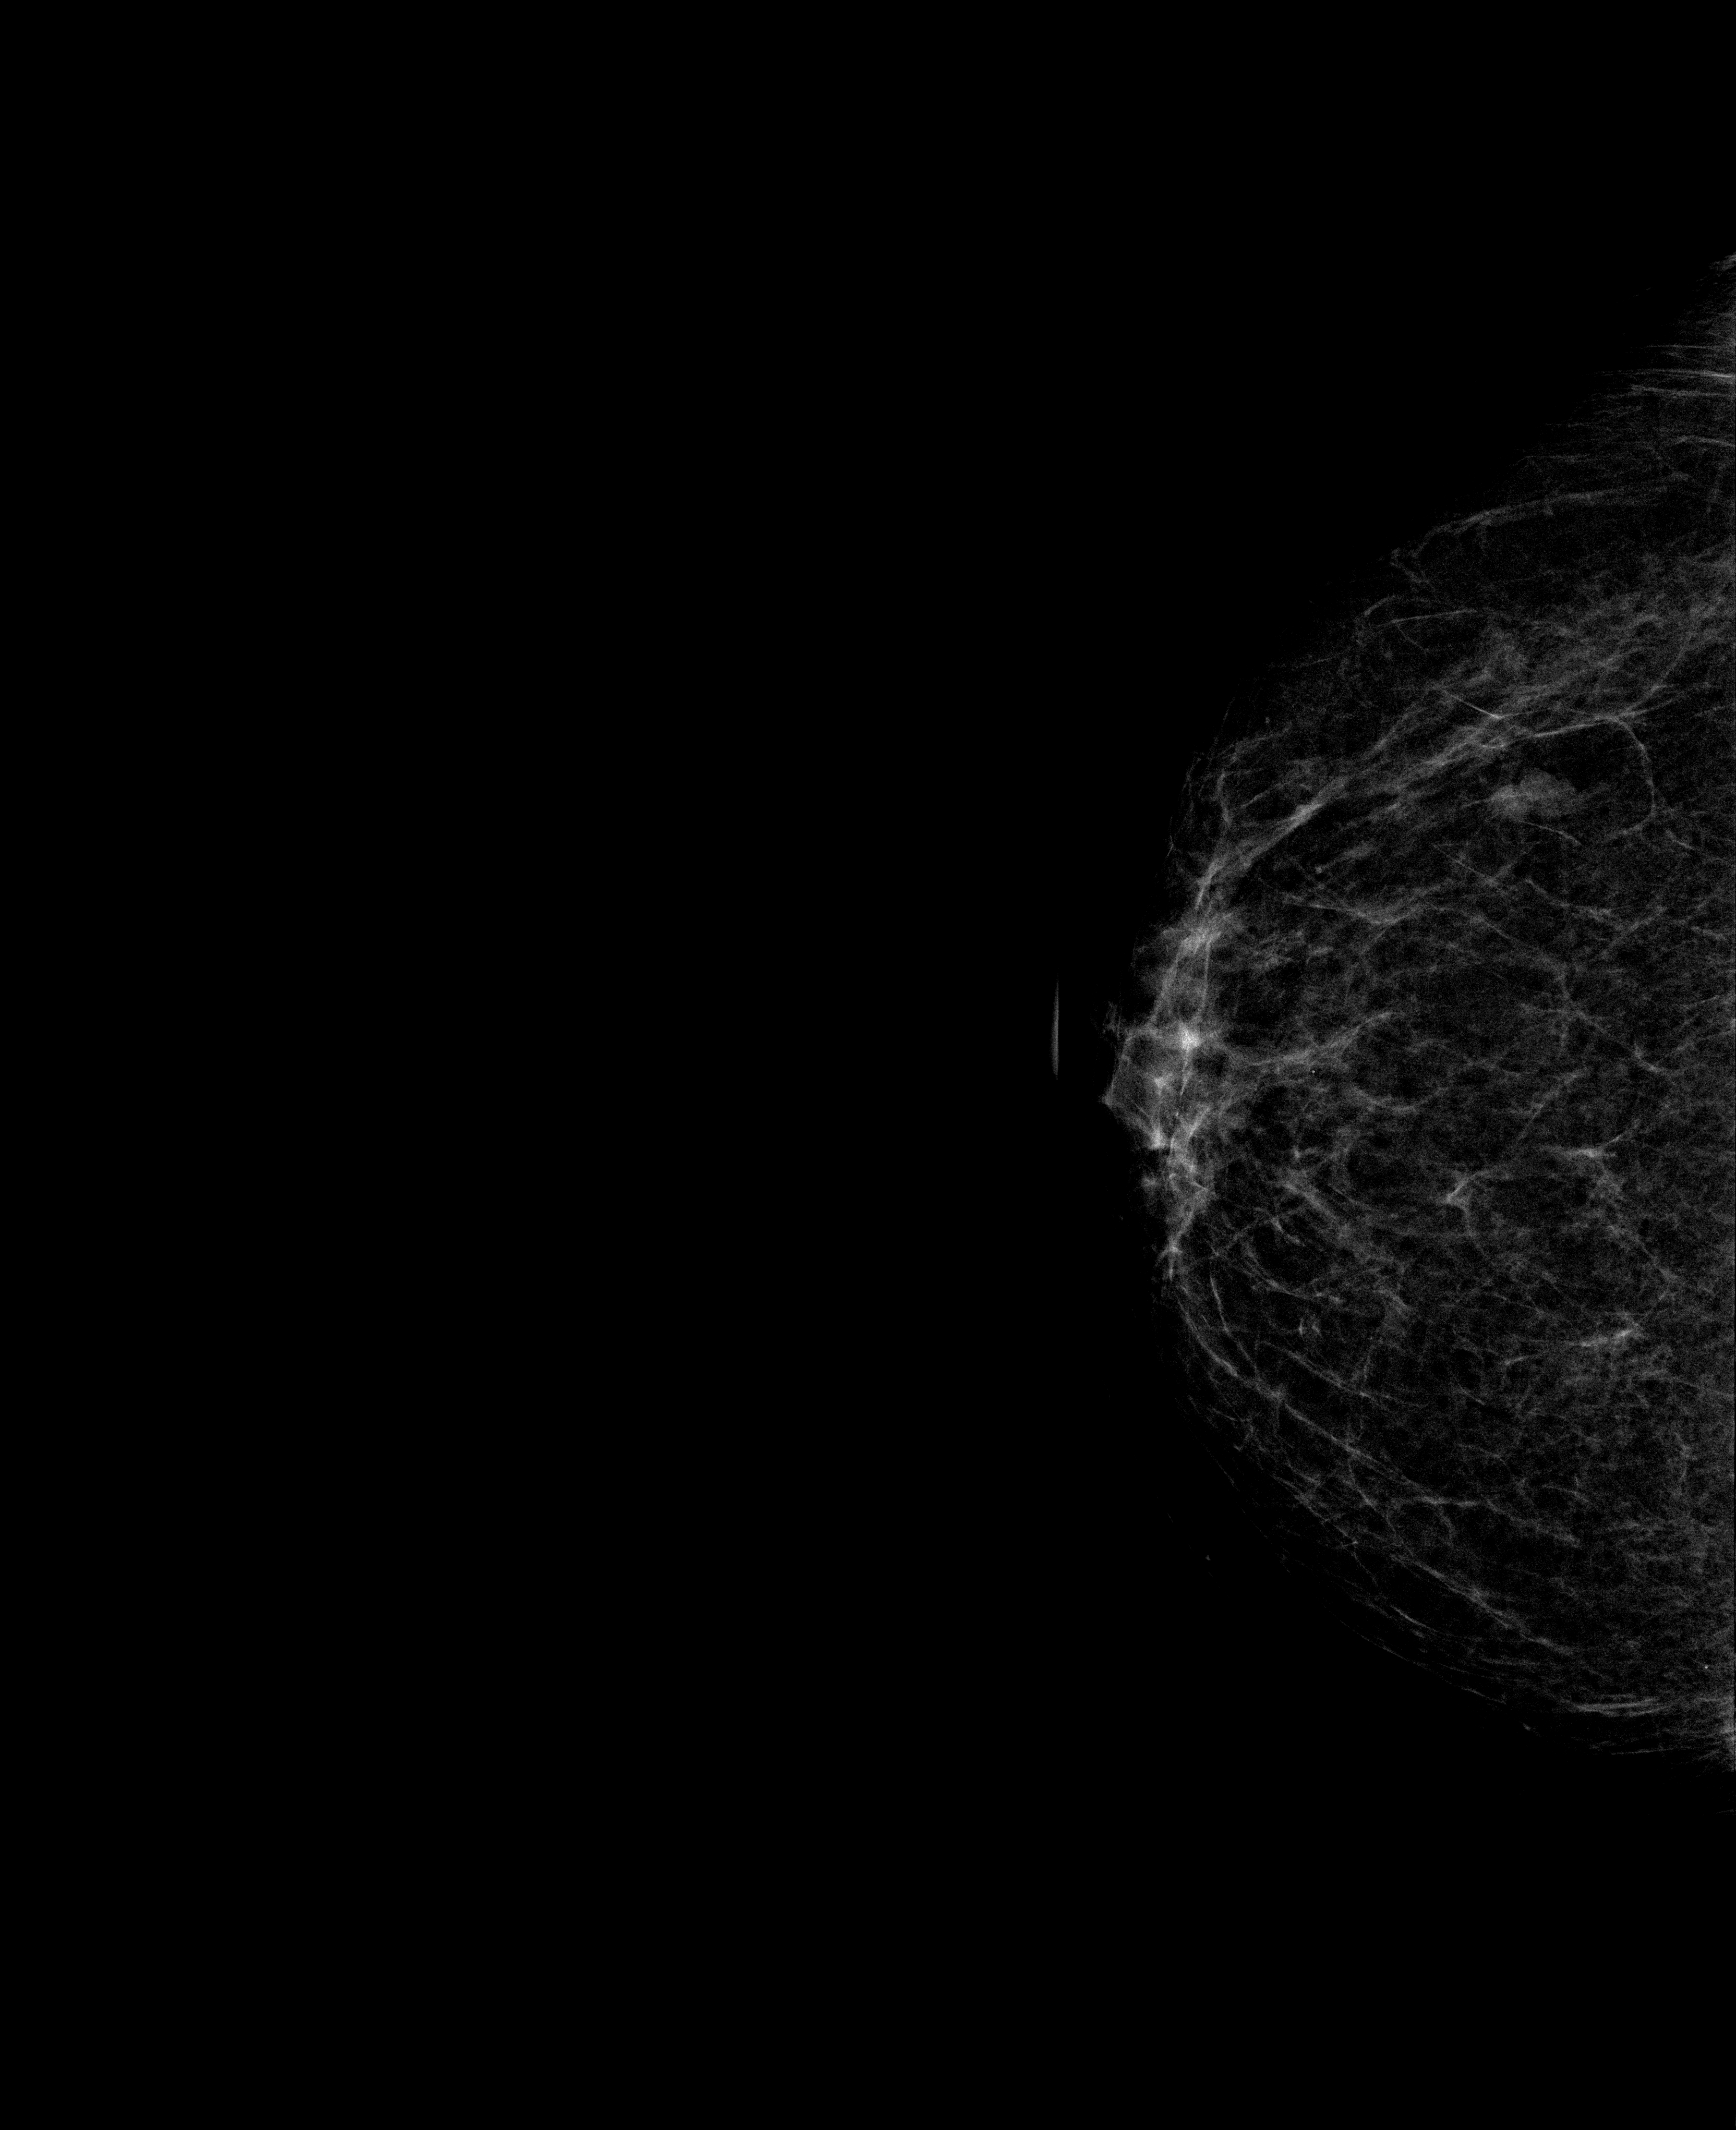
\includegraphics[height=3.5cm]{plots/mammogram_enhanced.png}
			\end{subfigure}
			\begin{subfigure}{0.24\textwidth}
				\centering
					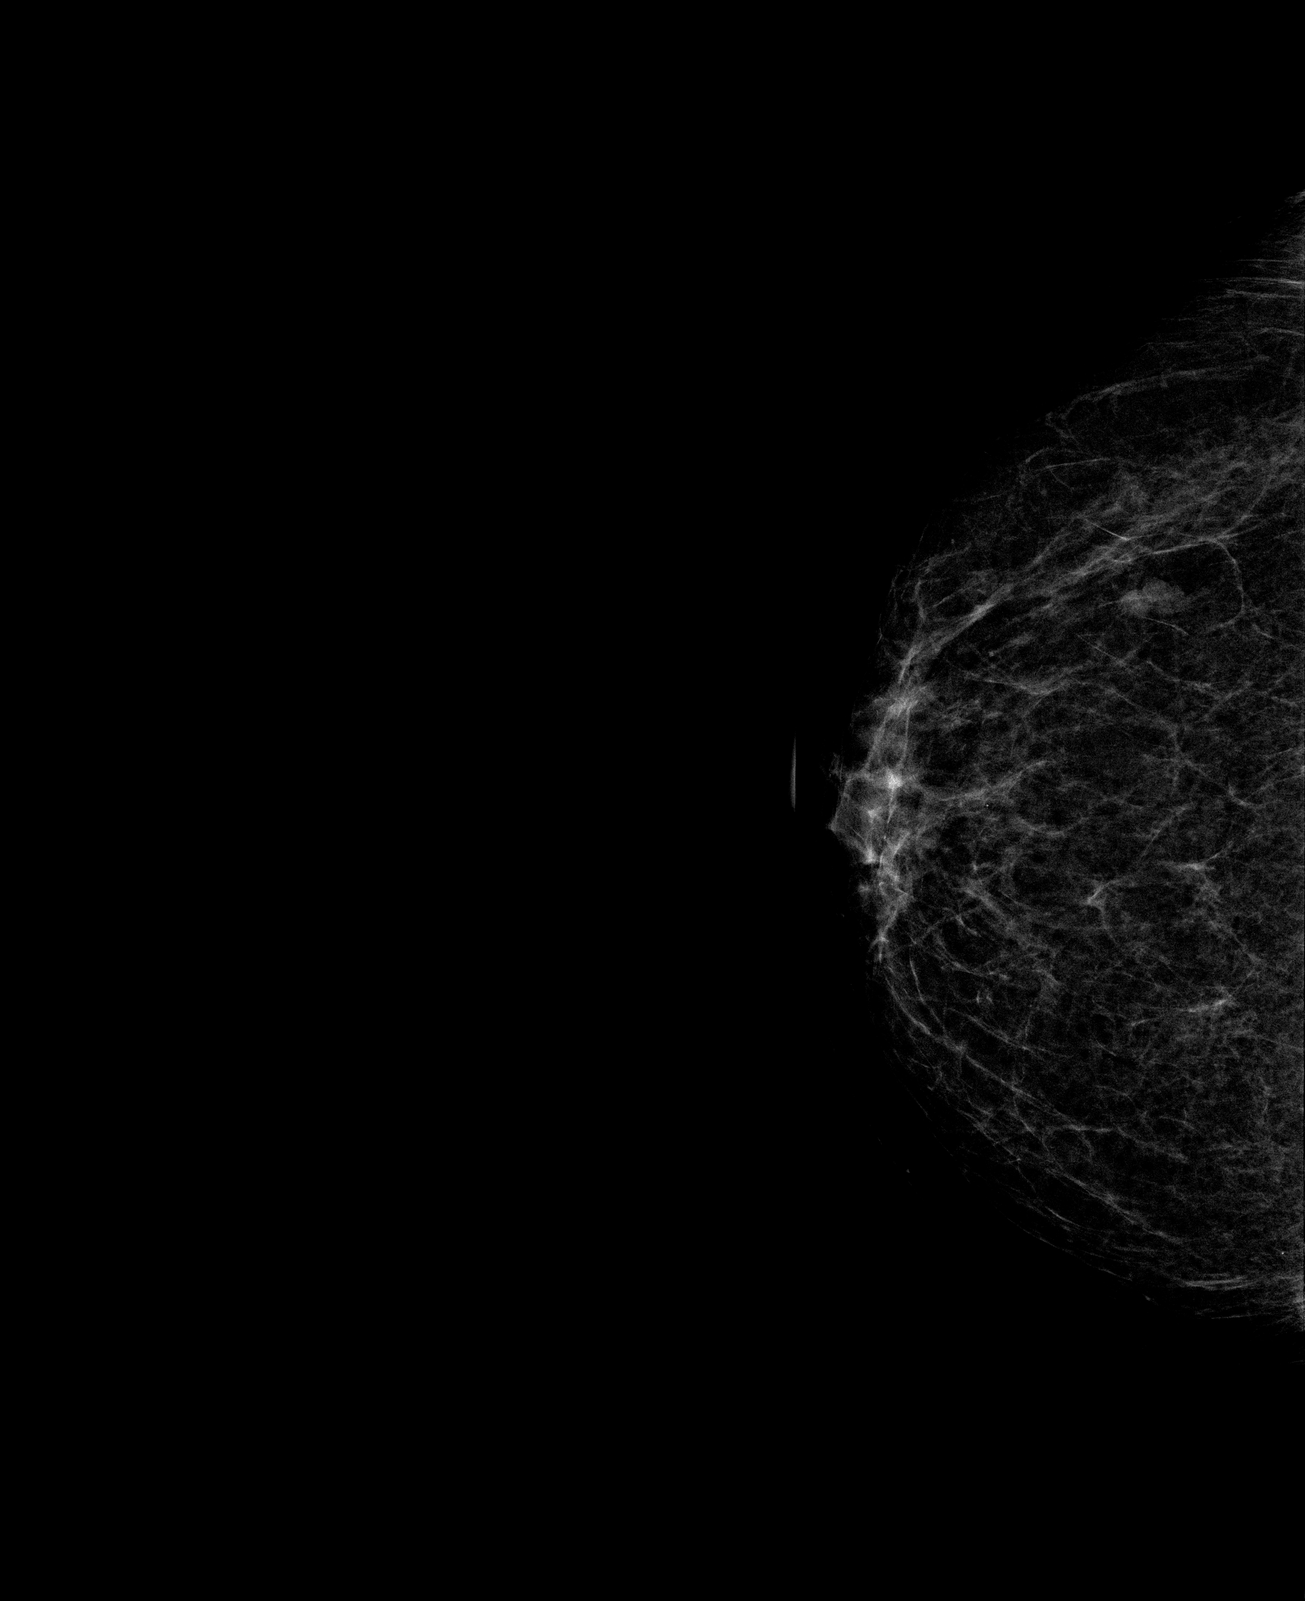
\includegraphics[height=3.5cm]{plots/mammogram_resized.png}
			\end{subfigure}
			\begin{subfigure}{0.11\textwidth}
				\centering
					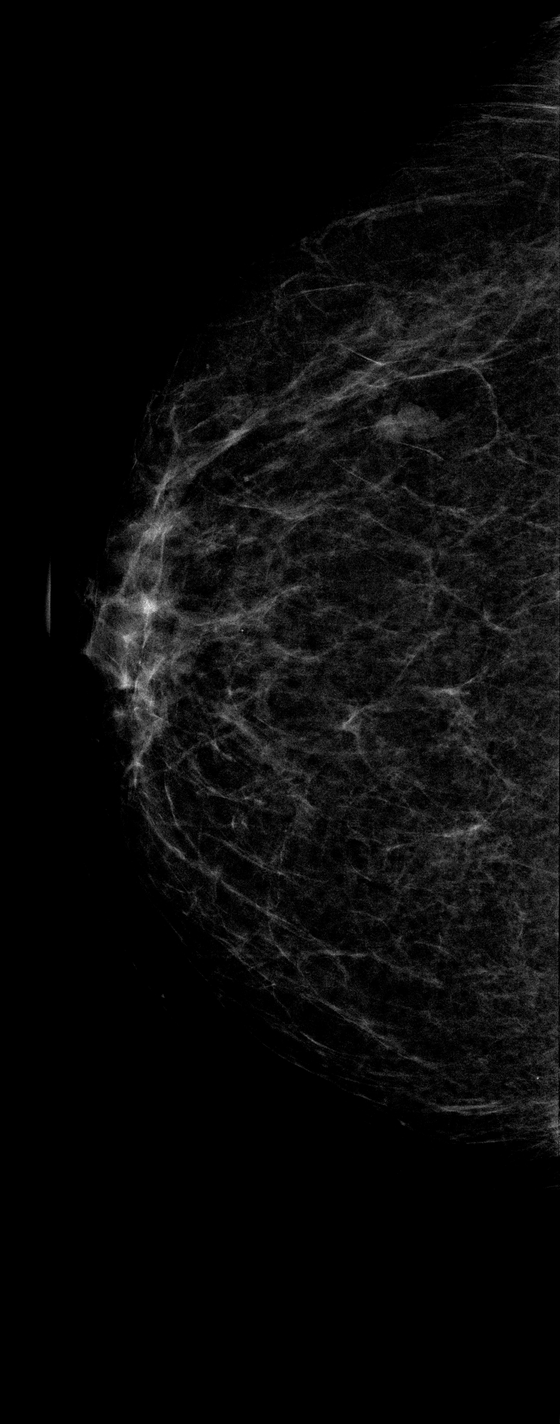
\includegraphics[height=3.5cm]{plots/mammogram_v1.png}
			\end{subfigure}
			~
			\begin{subfigure}{0.24\textwidth}
				\centering
					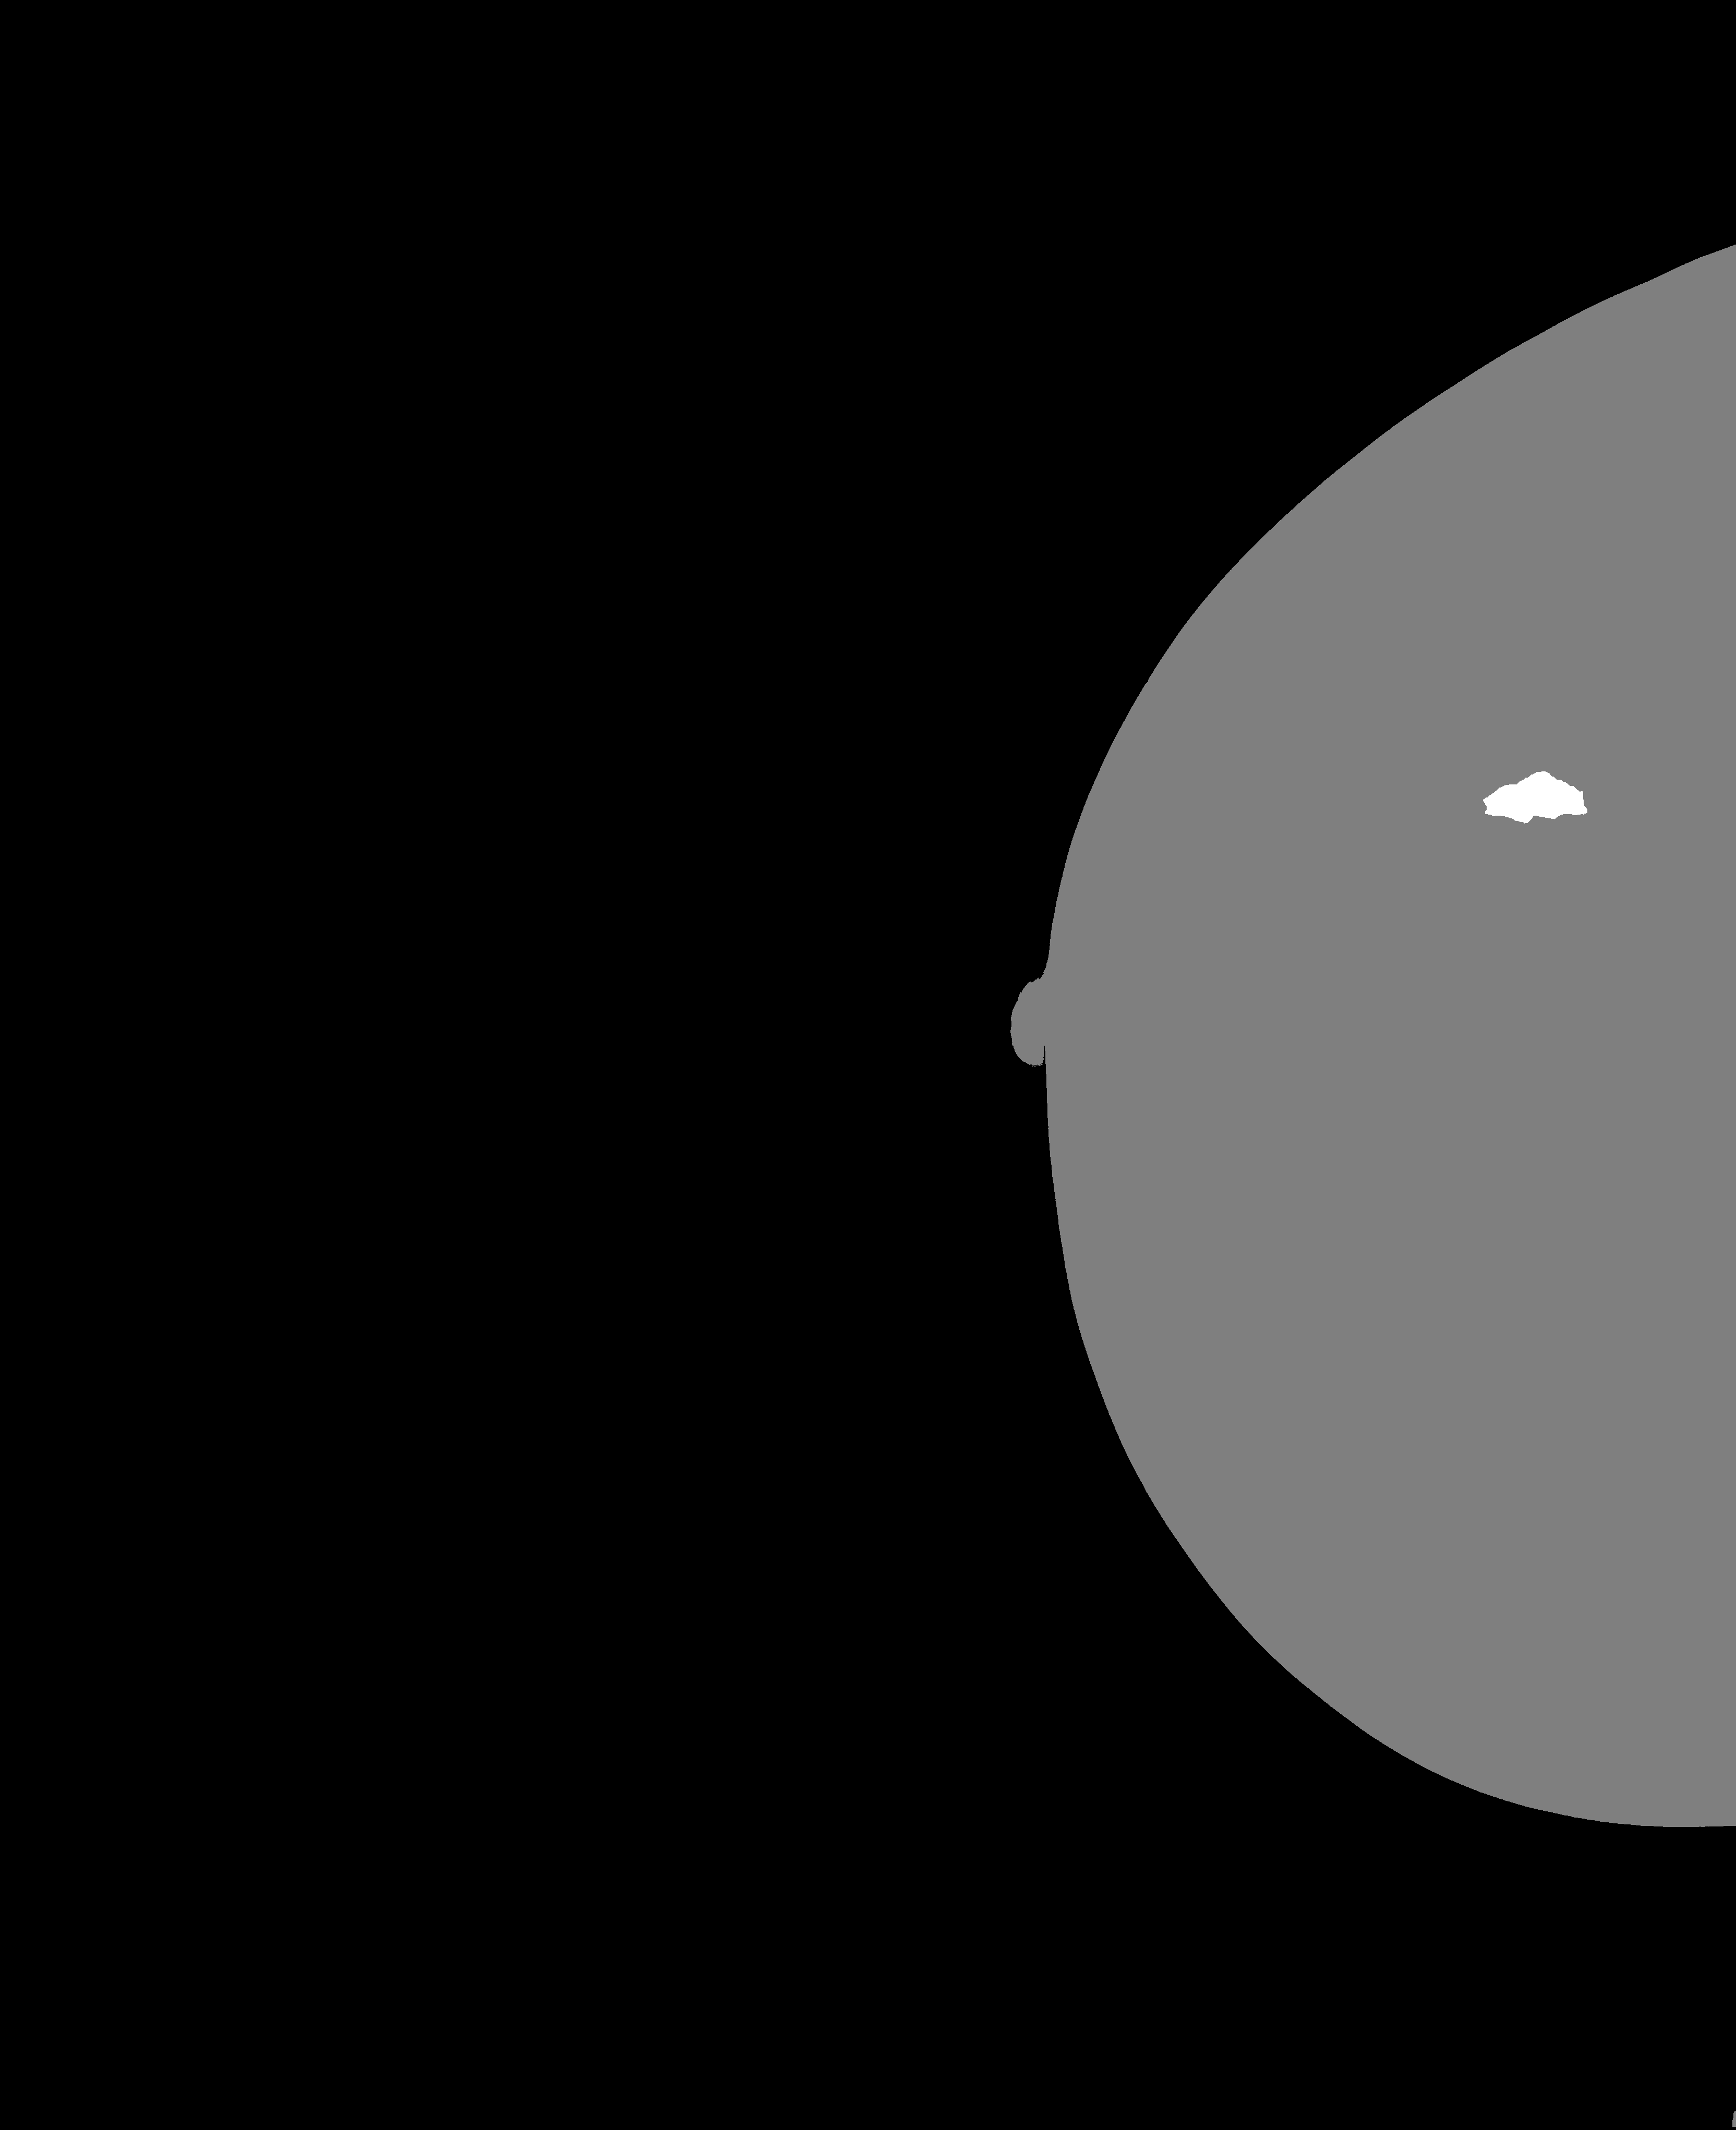
\includegraphics[height = 3.5cm]{plots/label.png}
				\caption{Original image}
				\label{subfig:Preprocessinga}
			\end{subfigure}
			\begin{subfigure}{0.24\textwidth}
				\centering
					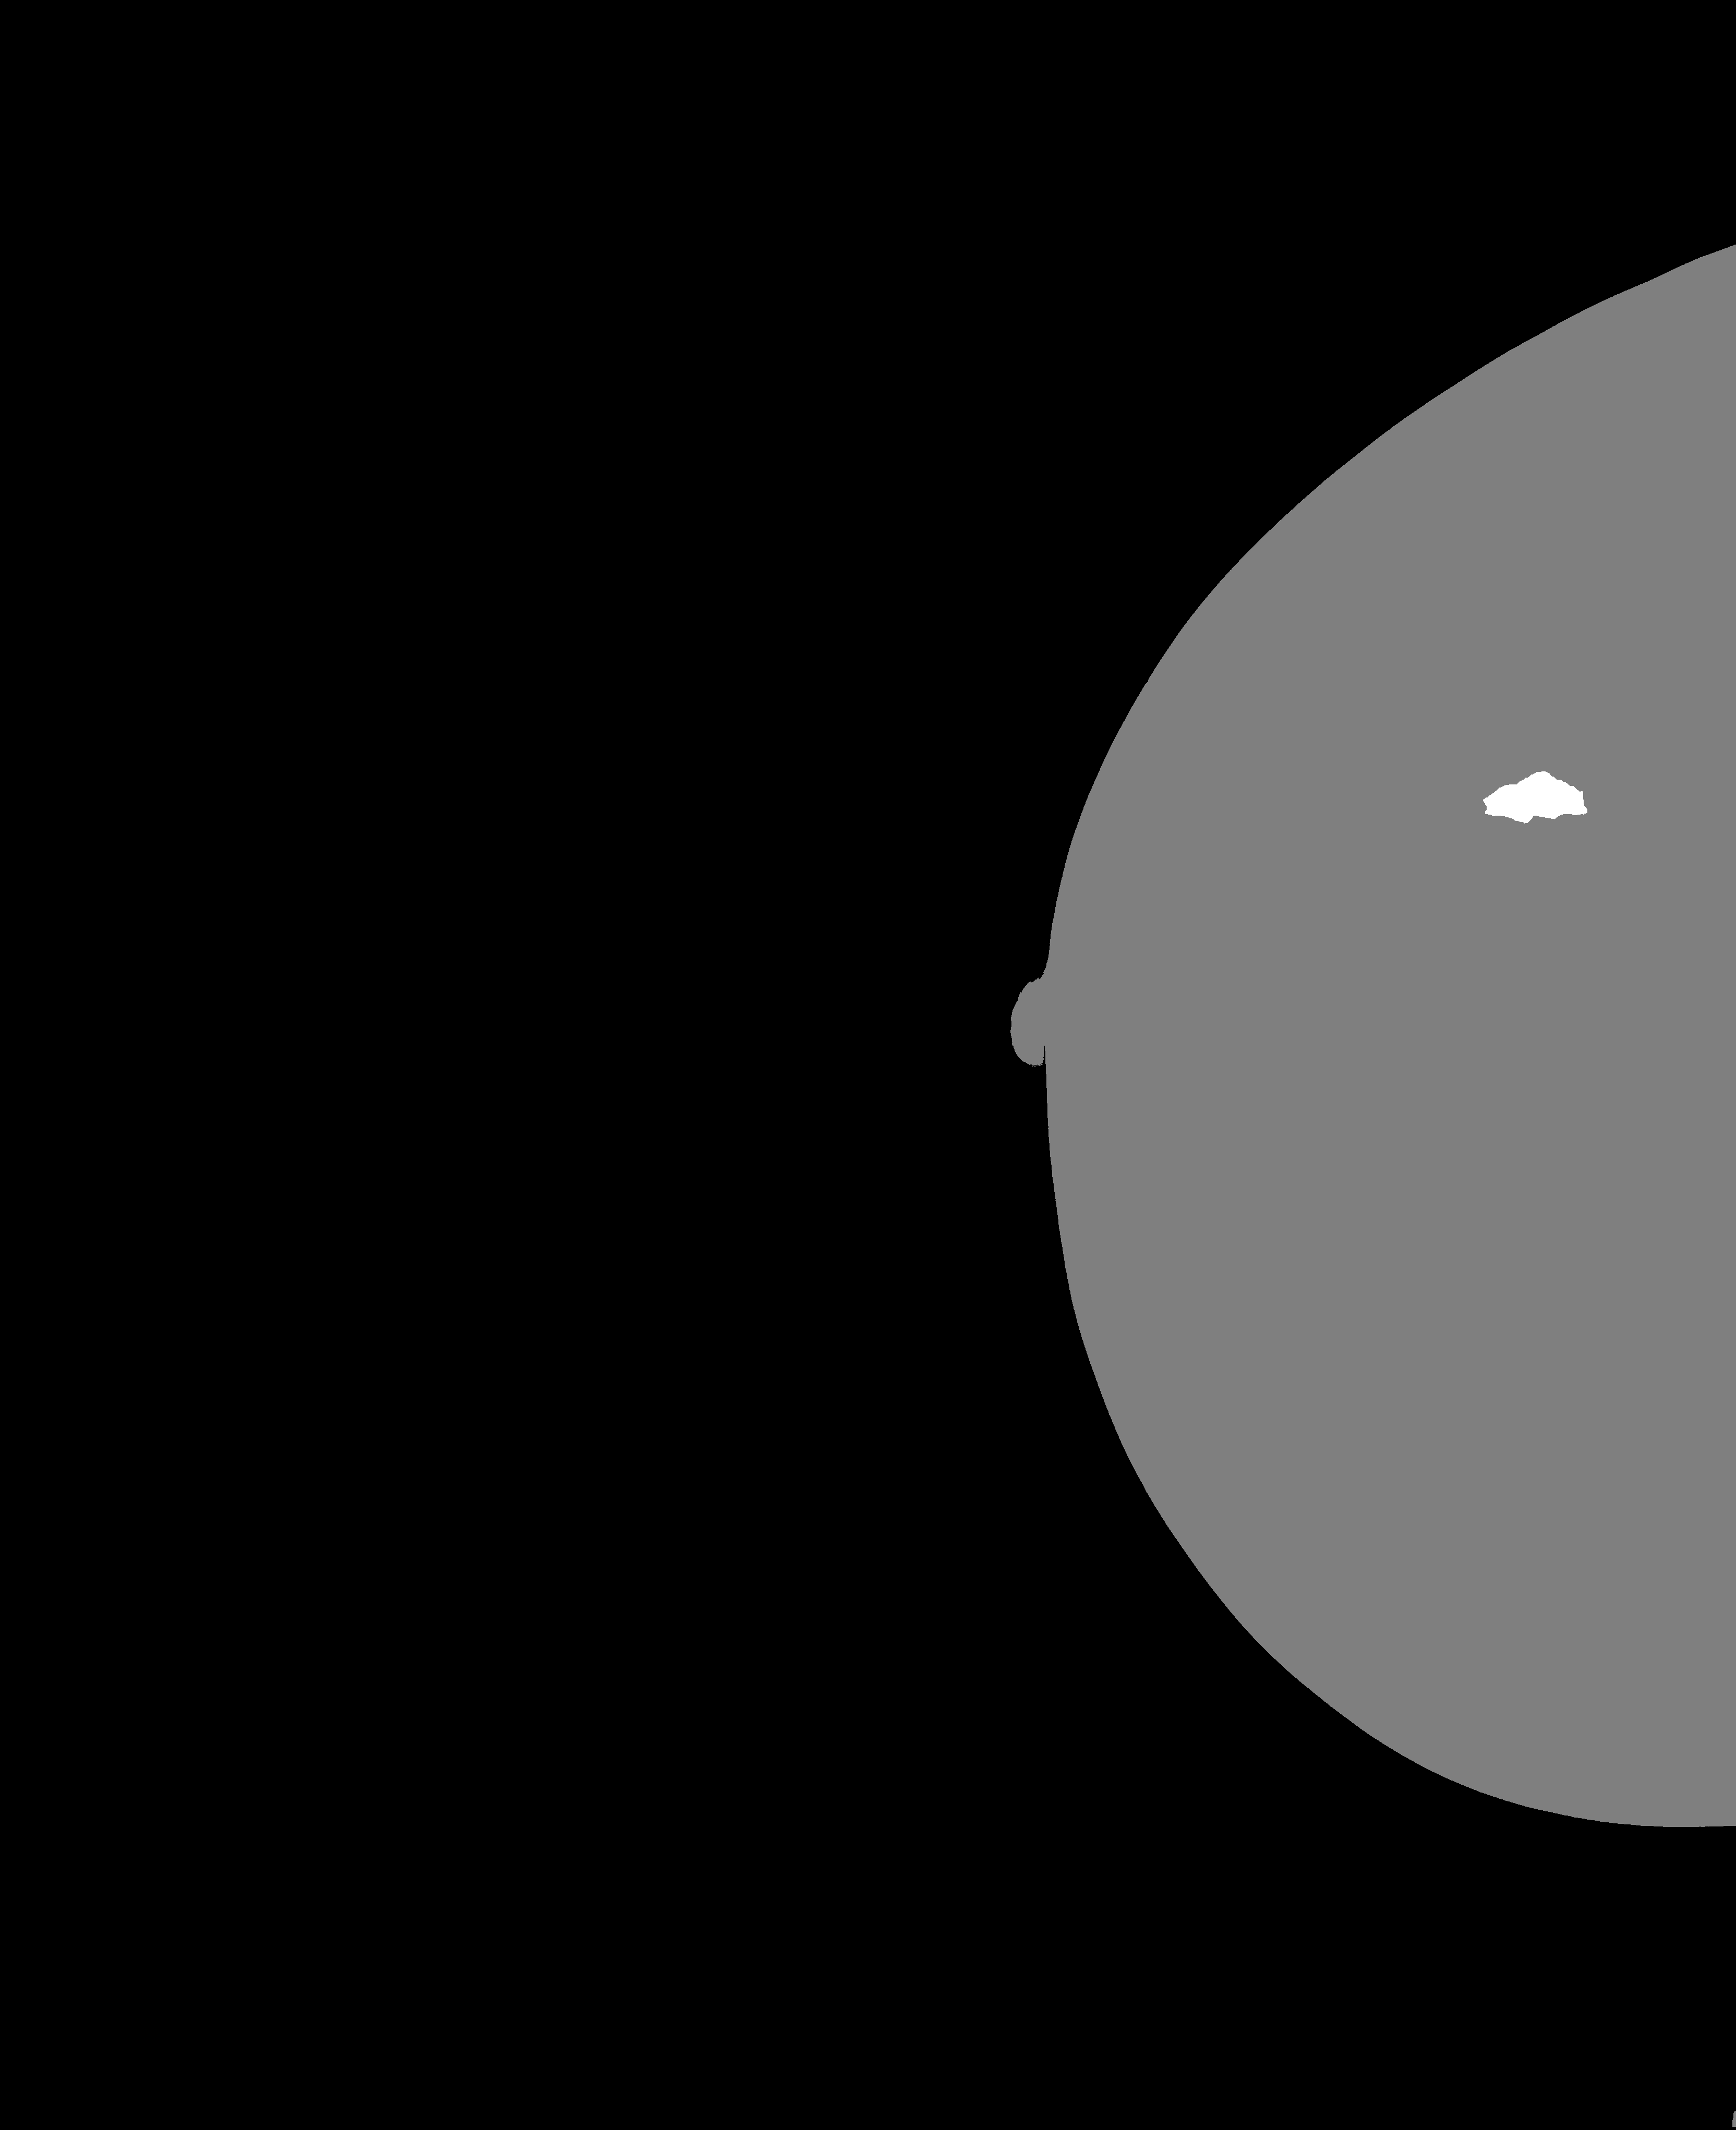
\includegraphics[height = 3.5cm]{plots/label_enhanced.png}
				\caption{Enhancement}
				\label{subfig:Preprocessingb}
			\end{subfigure}
			\begin{subfigure}{0.24\textwidth}
				\centering
					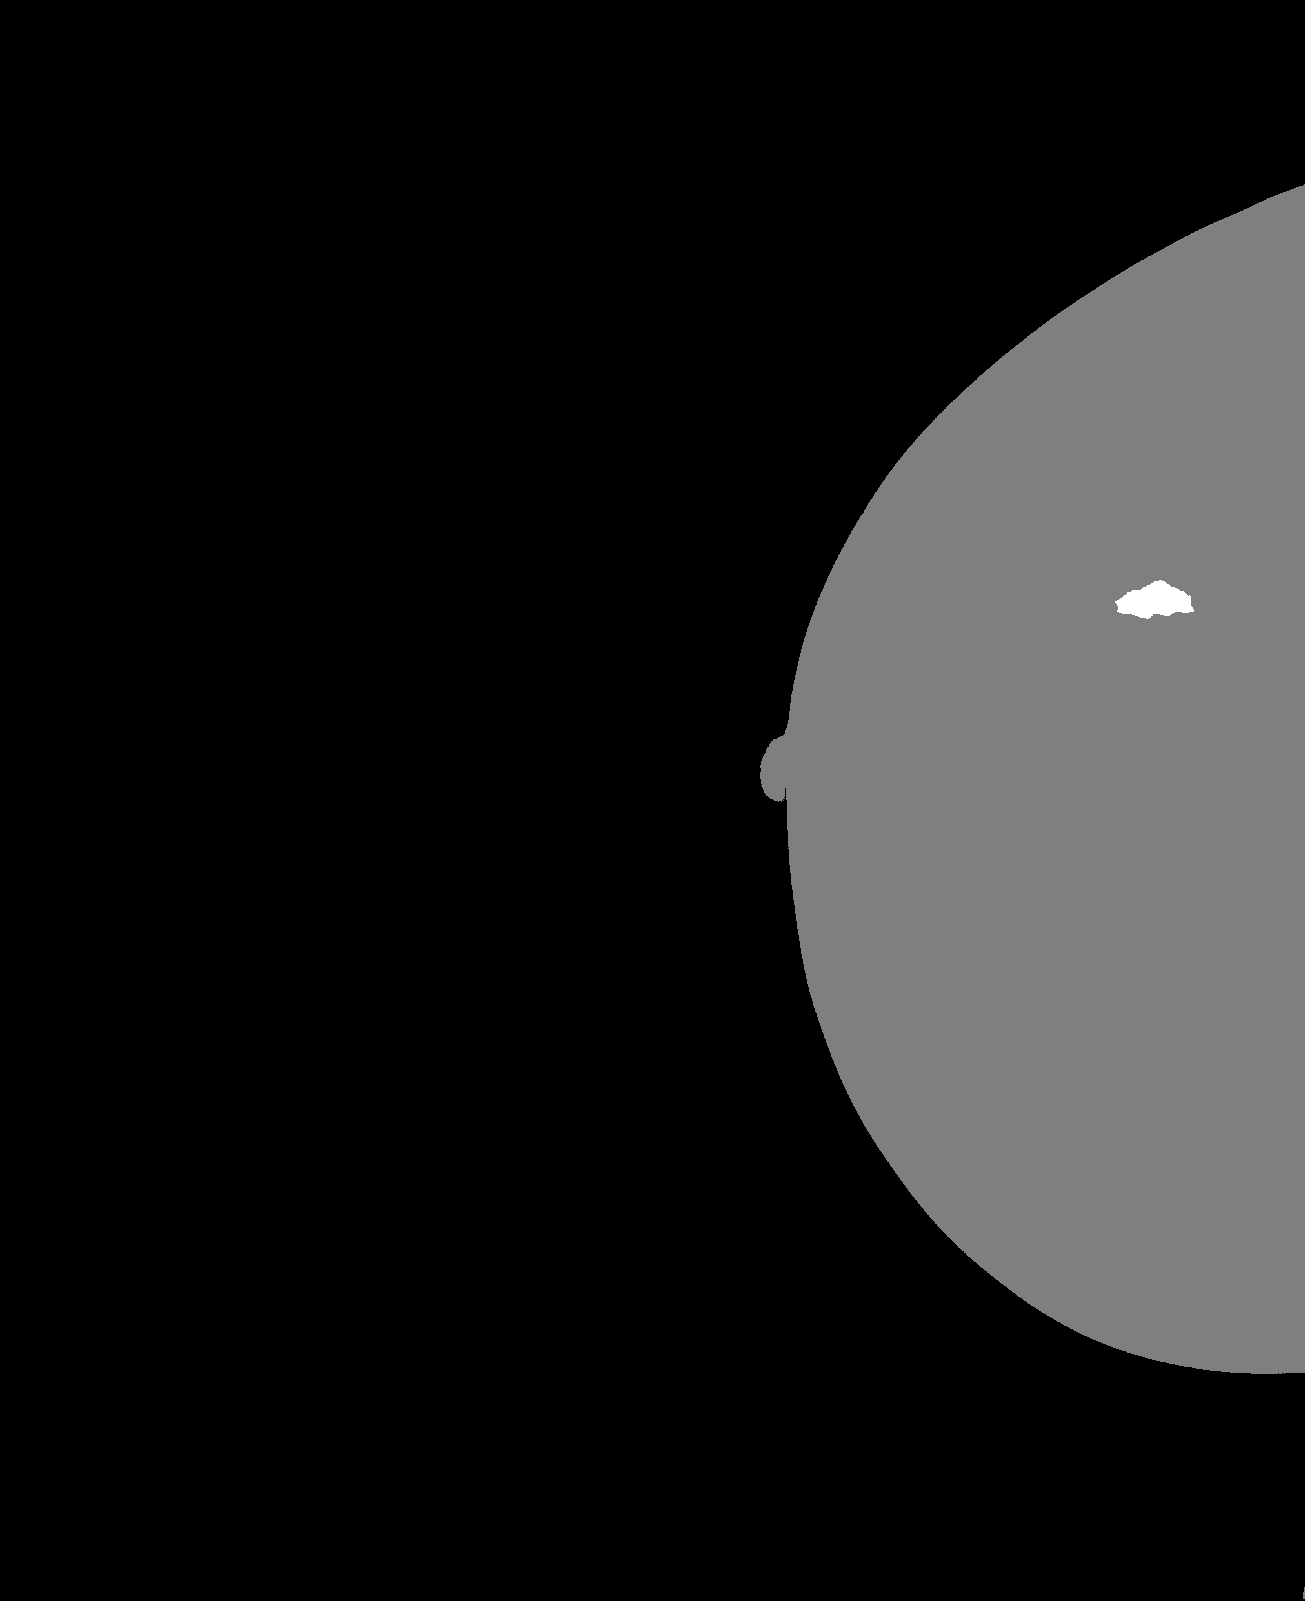
\includegraphics[height = 3.5cm]{plots/label_resized.png}
				\caption{Downsampling}
				\label{subfig:Preprocessingc}
			\end{subfigure}
			\begin{subfigure}{0.11\textwidth}
				\centering
					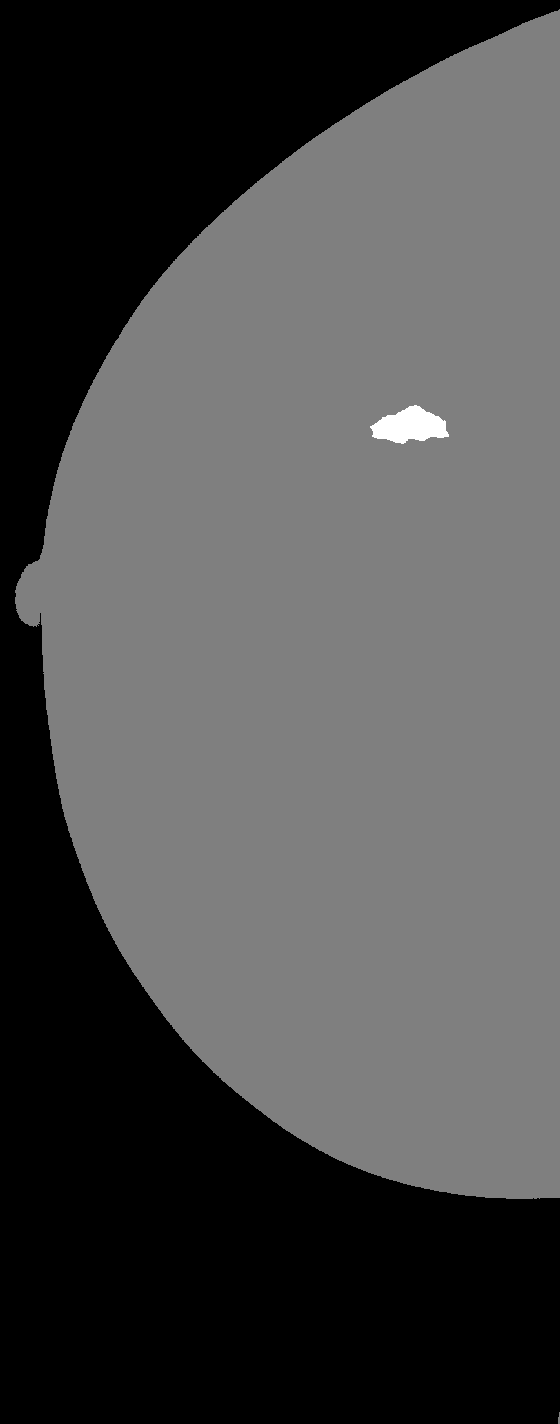
\includegraphics[height = 3.5cm]{plots/label_v1.png}
				\caption{Final}
				\label{subfig:Preprocessingd}
			\end{subfigure}
			% img_108_146_1_RCC.png
		\end{figure}
	\end{frame}
	
	\begin{frame}
		\frametitle{Software}
		\begin{figure}[h]
			\centering
			\begin{subfigure}{0.47\textwidth}
				\begin{subfigure}{\textwidth}
					
\includegraphics[width=\textwidth]{plots/tensorflow.png}
				\end{subfigure}
				\par \bigskip
				\begin{subfigure}{\textwidth}
					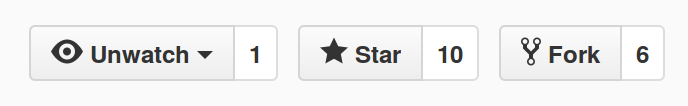
\includegraphics[width=\textwidth]{plots/github.png}
				\end{subfigure}
			\end{subfigure}
			~
			\begin{subfigure}{0.5\textwidth}
				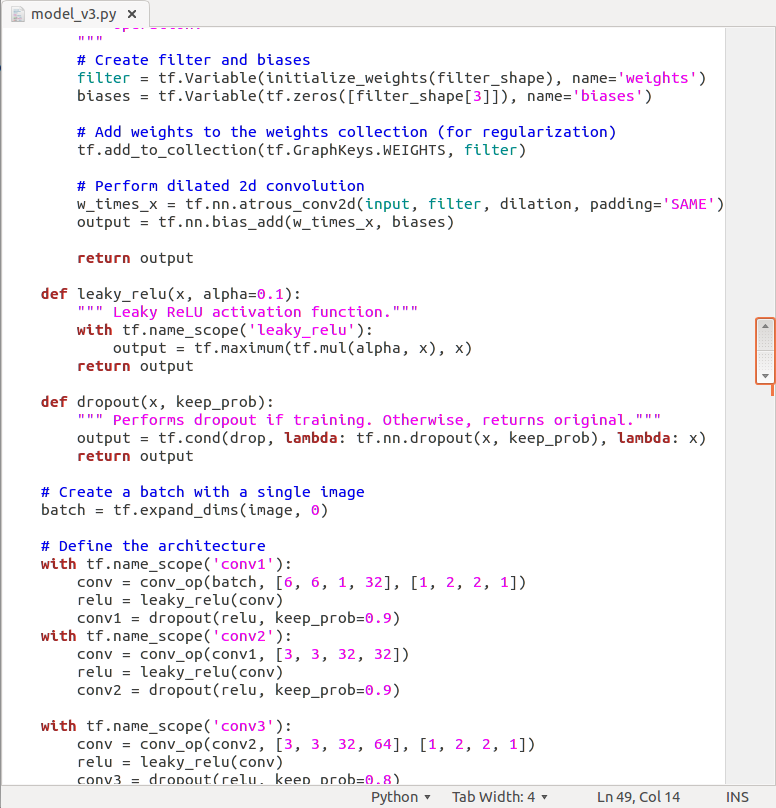
\includegraphics[width=\textwidth]{plots/code.png}
			\end{subfigure}
		\end{figure}
		%Seleccionar software, aprender tensorflow y havcer modelo.
	\end{frame}
	
	\begin{frame}
	\frametitle{Overview of the solution}
		\begin{figure}[ht]
			\centering
			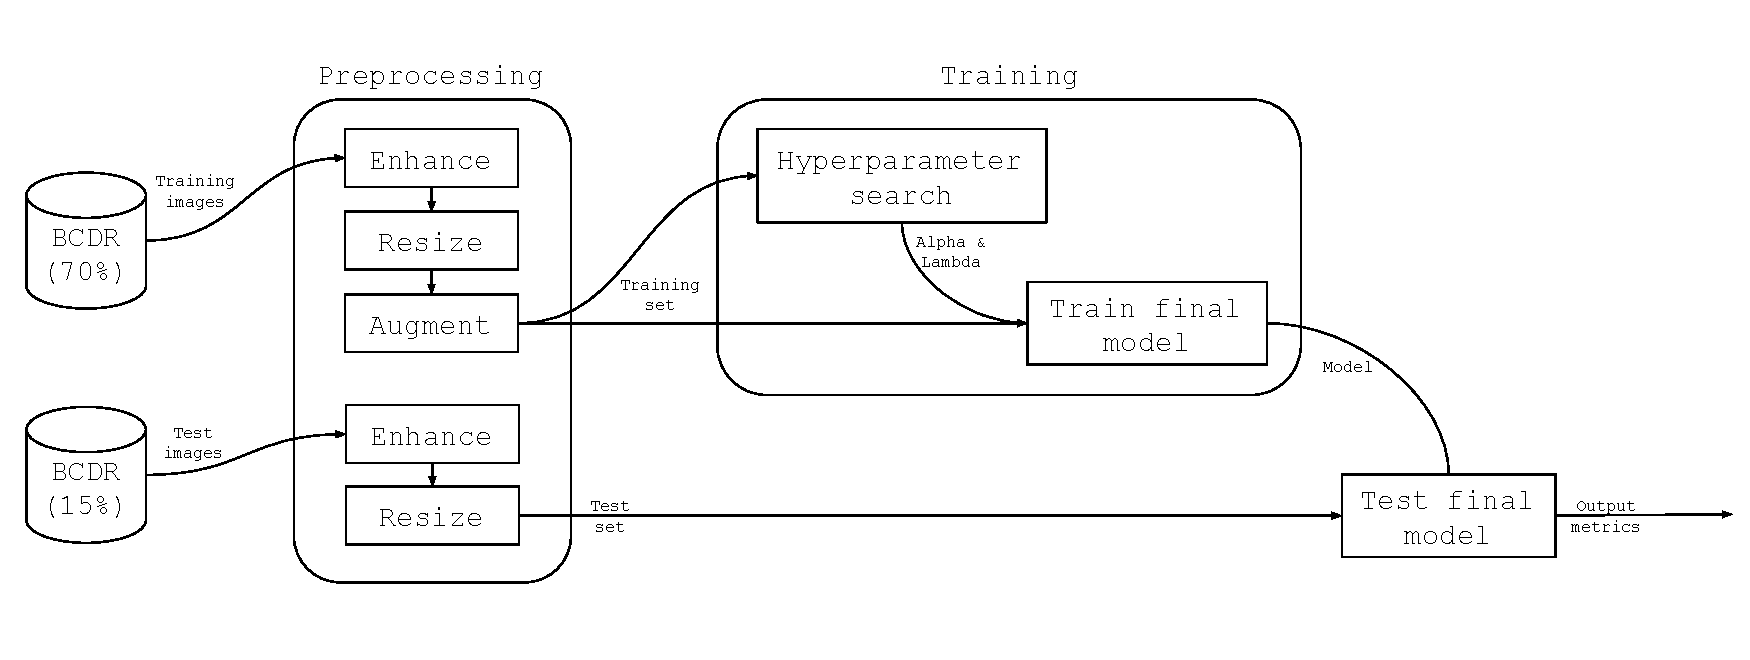
\includegraphics[width=\textwidth]{plots/overview.pdf}
		\end{figure}
	\end{frame}
	
	\begin{frame}
		\frametitle{Experiment 1}
		Modelled on a VGG network, winner of the 2014 ImageNet.
		% Say that it is like the Vgg-Net
		\footnotesize
		\begin{table}[h]
			\centering
			\begin{tabular}{lccccr}
			\hline
			\textbf{Layer} & \textbf{Filter} & \textbf{Stride} &\textbf{Pad} & \textbf{Volume} & \textbf{Parameters} \\
			\hline
			\texttt{INPUT}	& -	& - & - & $112 \times 112 \times 1$ & -\\
			\texttt{CONV -> Leaky RELU} & $6 \times 6$ & 2 & 2 & $56 \times 56 \times 56$ & 2\,072\\
			\texttt{CONV -> Leaky RELU} & $3 \times 3$ & 1 & 1 & $56 \times 56 \times 56$ & 28\,280\\
			\texttt{MAXPOOL} & $2 \times 2$ & 2 & 0 & $28 \times 28 \times 56$ & -\\
			\texttt{CONV -> Leaky RELU} & $3 \times 3$ & 1 & 1 & $28 \times 28 \times 84$ & 42\,420\\
			\texttt{CONV -> Leaky RELU} & $3 \times 3$ & 1 & 1 & $28 \times 28 \times 84$ & 63\,588\\
			\texttt{MAXPOOL} & $2 \times 2$ & 2 & 0 & $14 \times 14 \times 84$ & -\\
			\texttt{CONV -> Leaky RELU} & $3 \times 3$ & 1 & 1 & $14 \times 14 \times 112$ & 84\,784\\
			\texttt{CONV -> Leaky RELU} & $3 \times 3$ & 1 & 1 & $14 \times 14 \times 112$ & 113\,008\\
			\texttt{CONV -> Leaky RELU} & $3 \times 3$ & 1 & 1 & $14 \times 14 \times 112$ & 113\,008\\
			\texttt{MAXPOOL} & $2 \times 2$ & 2 & 0 & $7 \times 7 \times 112$ & -\\
			\texttt{FC -> Leaky RELU} & $7 \times 7$ & 1 & 3 & $7 \times 7 \times 448$ & 2\,459\,072\\
			\texttt{FC} & $1 \times 1$ & 1 & 0 & $7 \times 7 \times 1$ & 449 \\
			\texttt{BILINEAR (x16)} & - & - & - & $112 \times 112 \times 1$ & -\\
			\hline
			\end{tabular}
		\end{table}
		
		\scriptsize
		\begin{table}[h]
			\centering
			\begin{tabular}{cccccccc}
			\hline
			\textbf{IOU}	& \textbf{F1-score}	& \textbf{G-mean} &\textbf{Accuracy}	& \textbf{Sensitivity} & \textbf{Specificity} & \textbf{Precision} & \textbf{Recall}\\
			\hline
			0.109 & 0.197 & 0.49 & 0.98 & 0.243 & 0.987 & 0.165 & 0.243 \\
			\hline
			\end{tabular}
		\end{table}

	\end{frame}

	\begin{frame}
		\frametitle{Qualitative results}
		\begin{figure}[h]
		\centering
			\begin{subfigure}{0.25\textwidth}
				\centering
					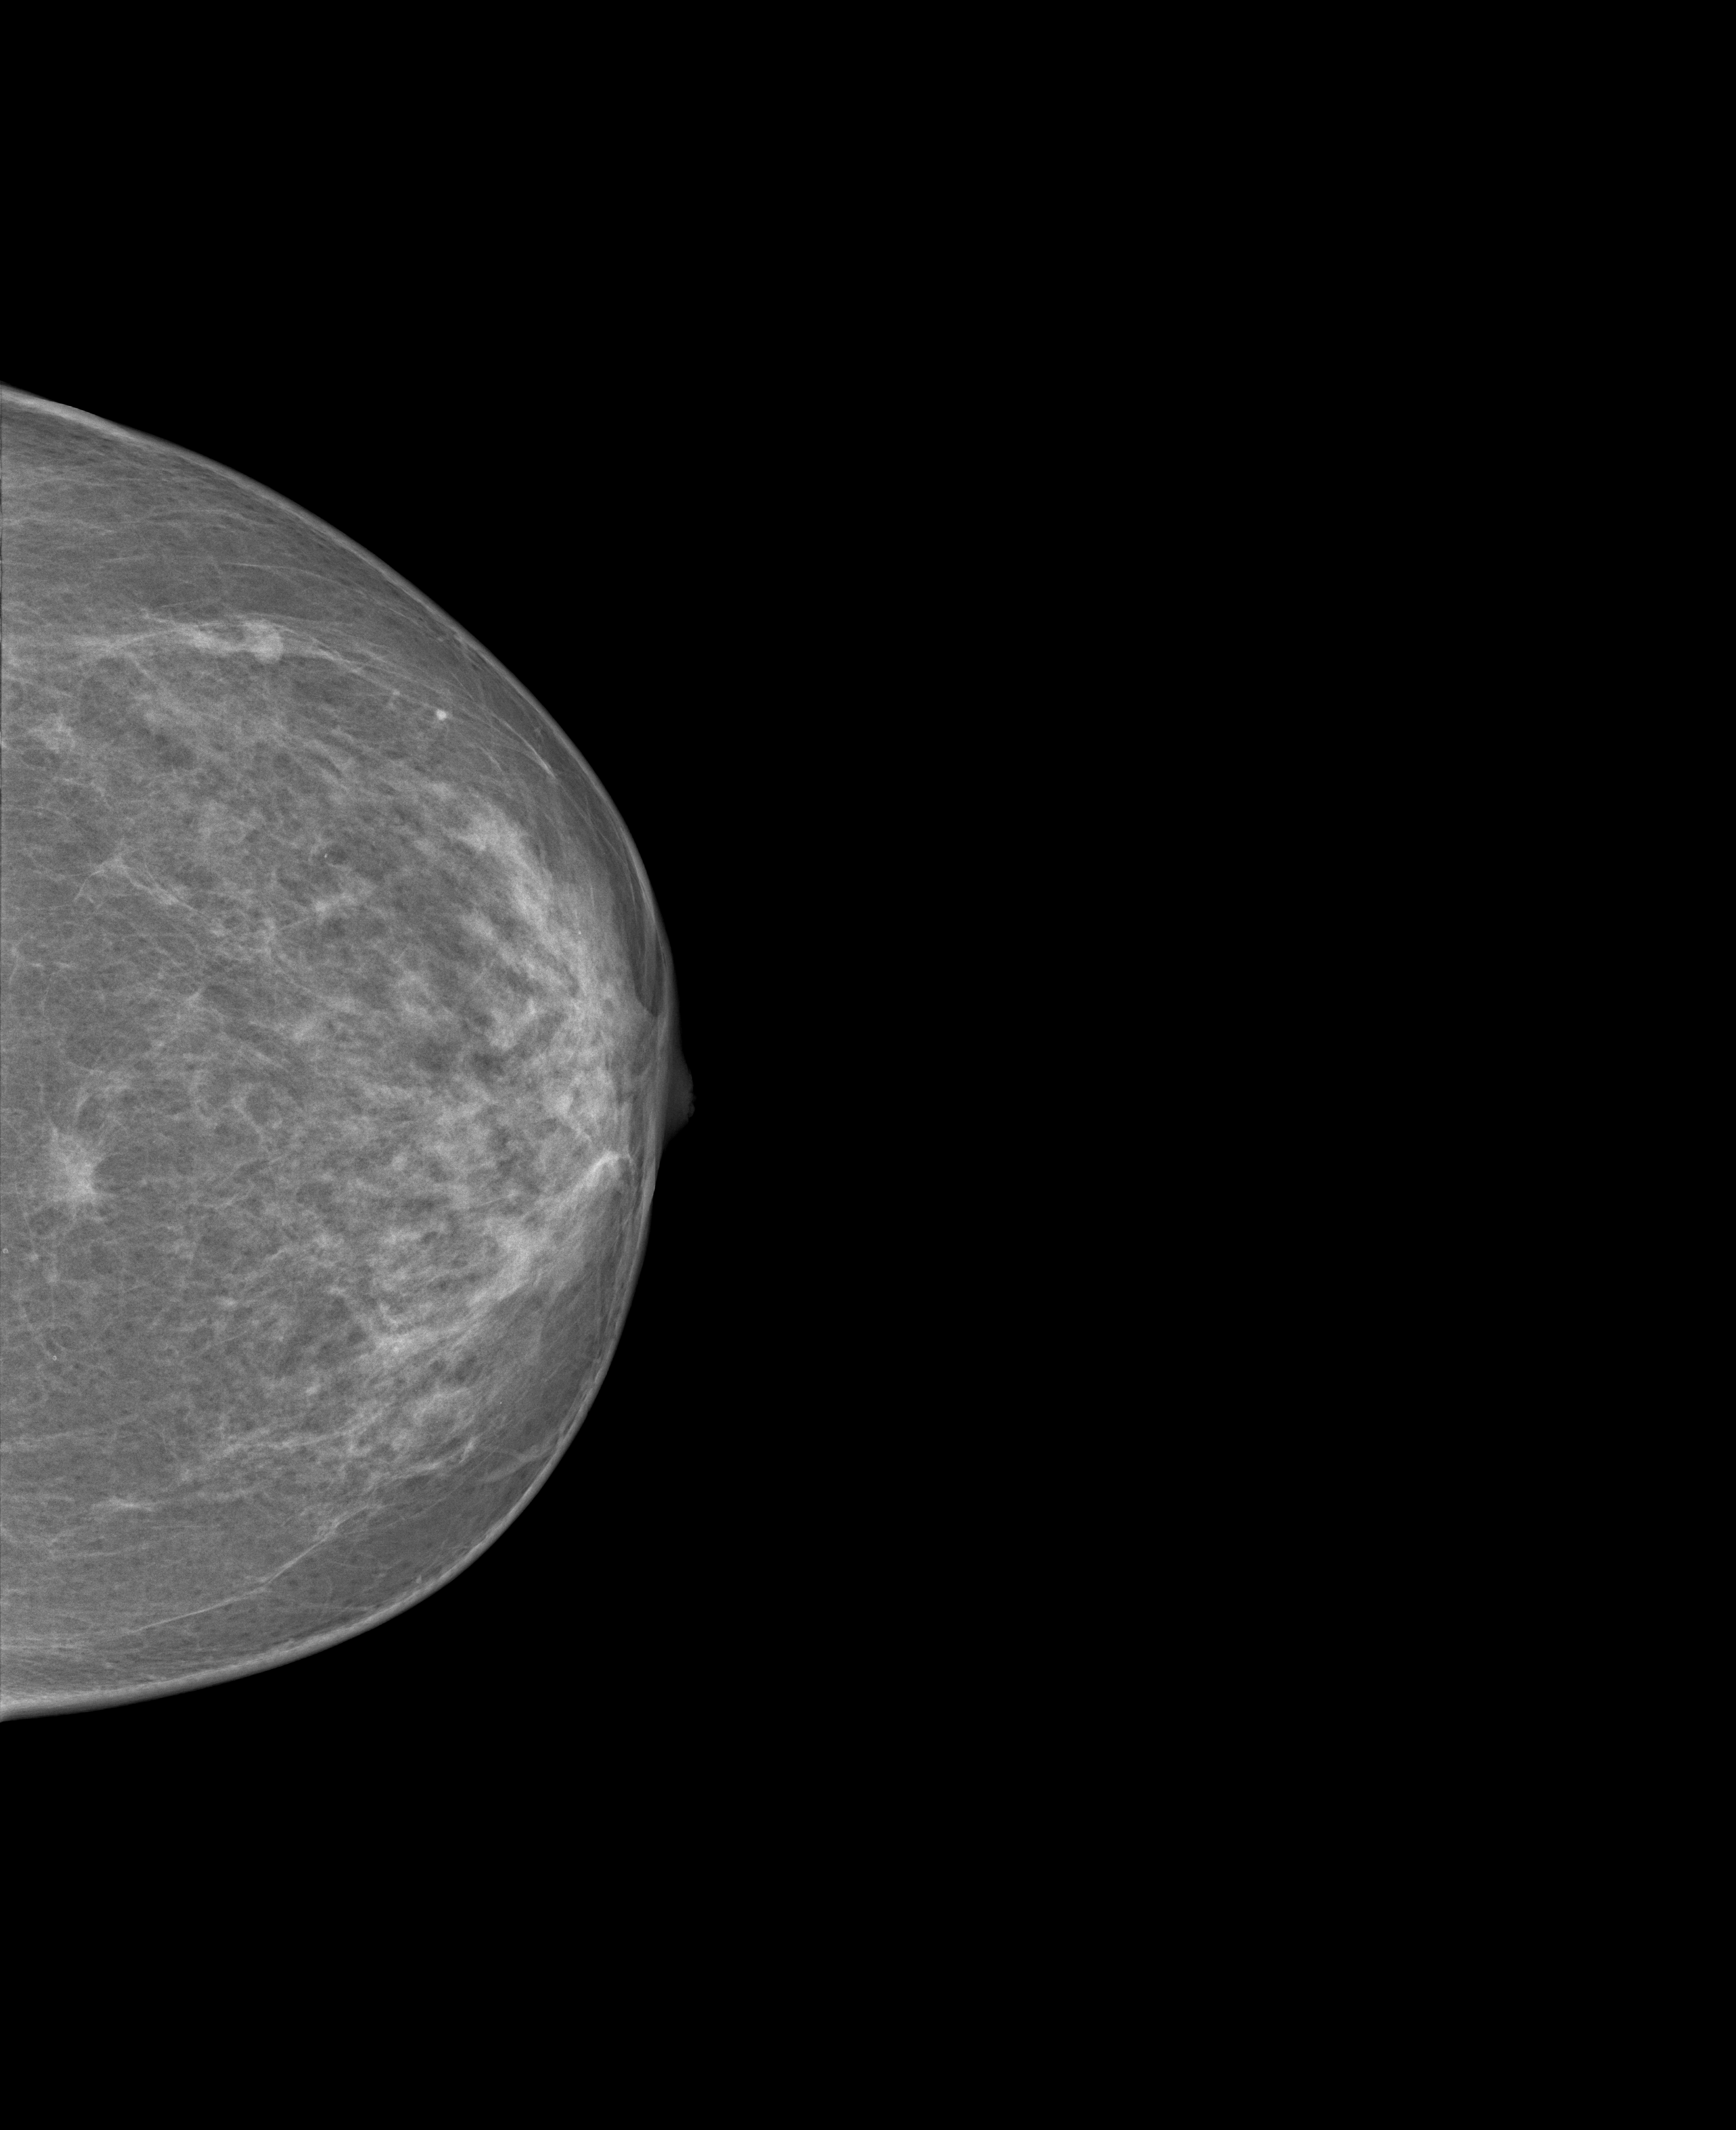
\includegraphics[height=3.5cm]{plots/mammogram_ex1.png}
			\end{subfigure}
			\begin{subfigure}{0.16\textwidth}
				\centering
					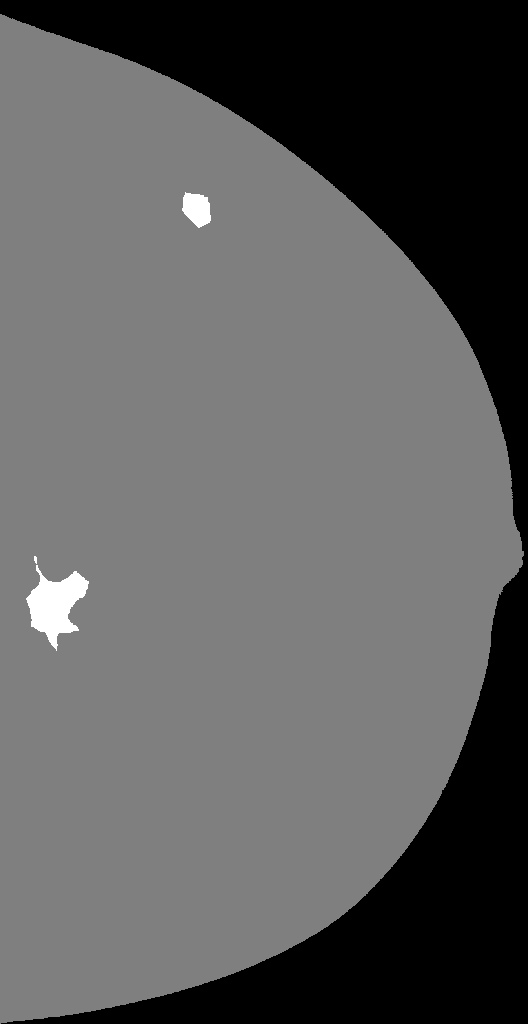
\includegraphics[height=3.5cm]{plots/label_ex1.png}
			\end{subfigure}
			\begin{subfigure}{0.17\textwidth}
				\centering
					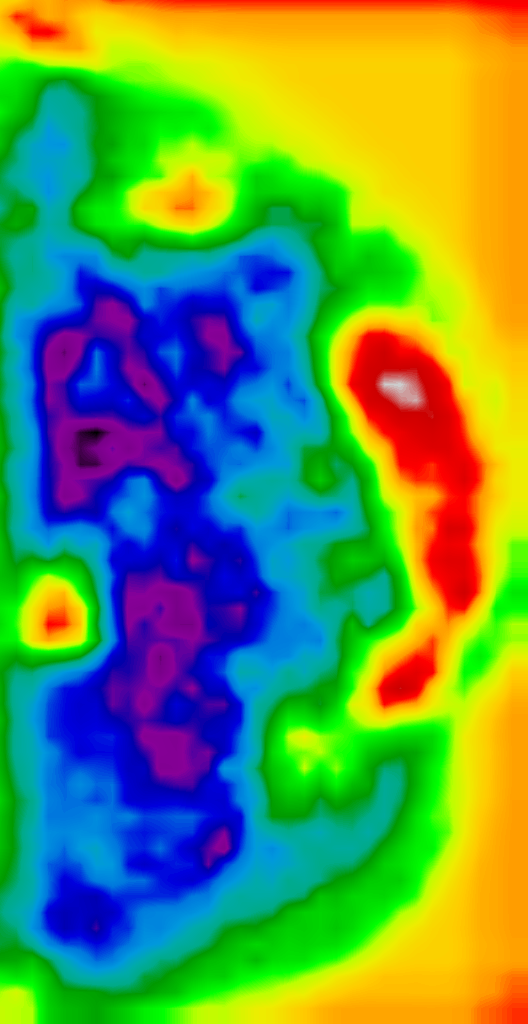
\includegraphics[height=3.5cm]{plots/logits_ex1_v1.png}
			\end{subfigure}
			\begin{subfigure}{0.22\textwidth}
				\centering
					
\includegraphics[height=3.5cm]{plots/segmentation_ex1_v1.png}
			\end{subfigure}%img_251_334_1_LCC.png
			\\
			\begin{subfigure}{0.25\textwidth}
				\centering
					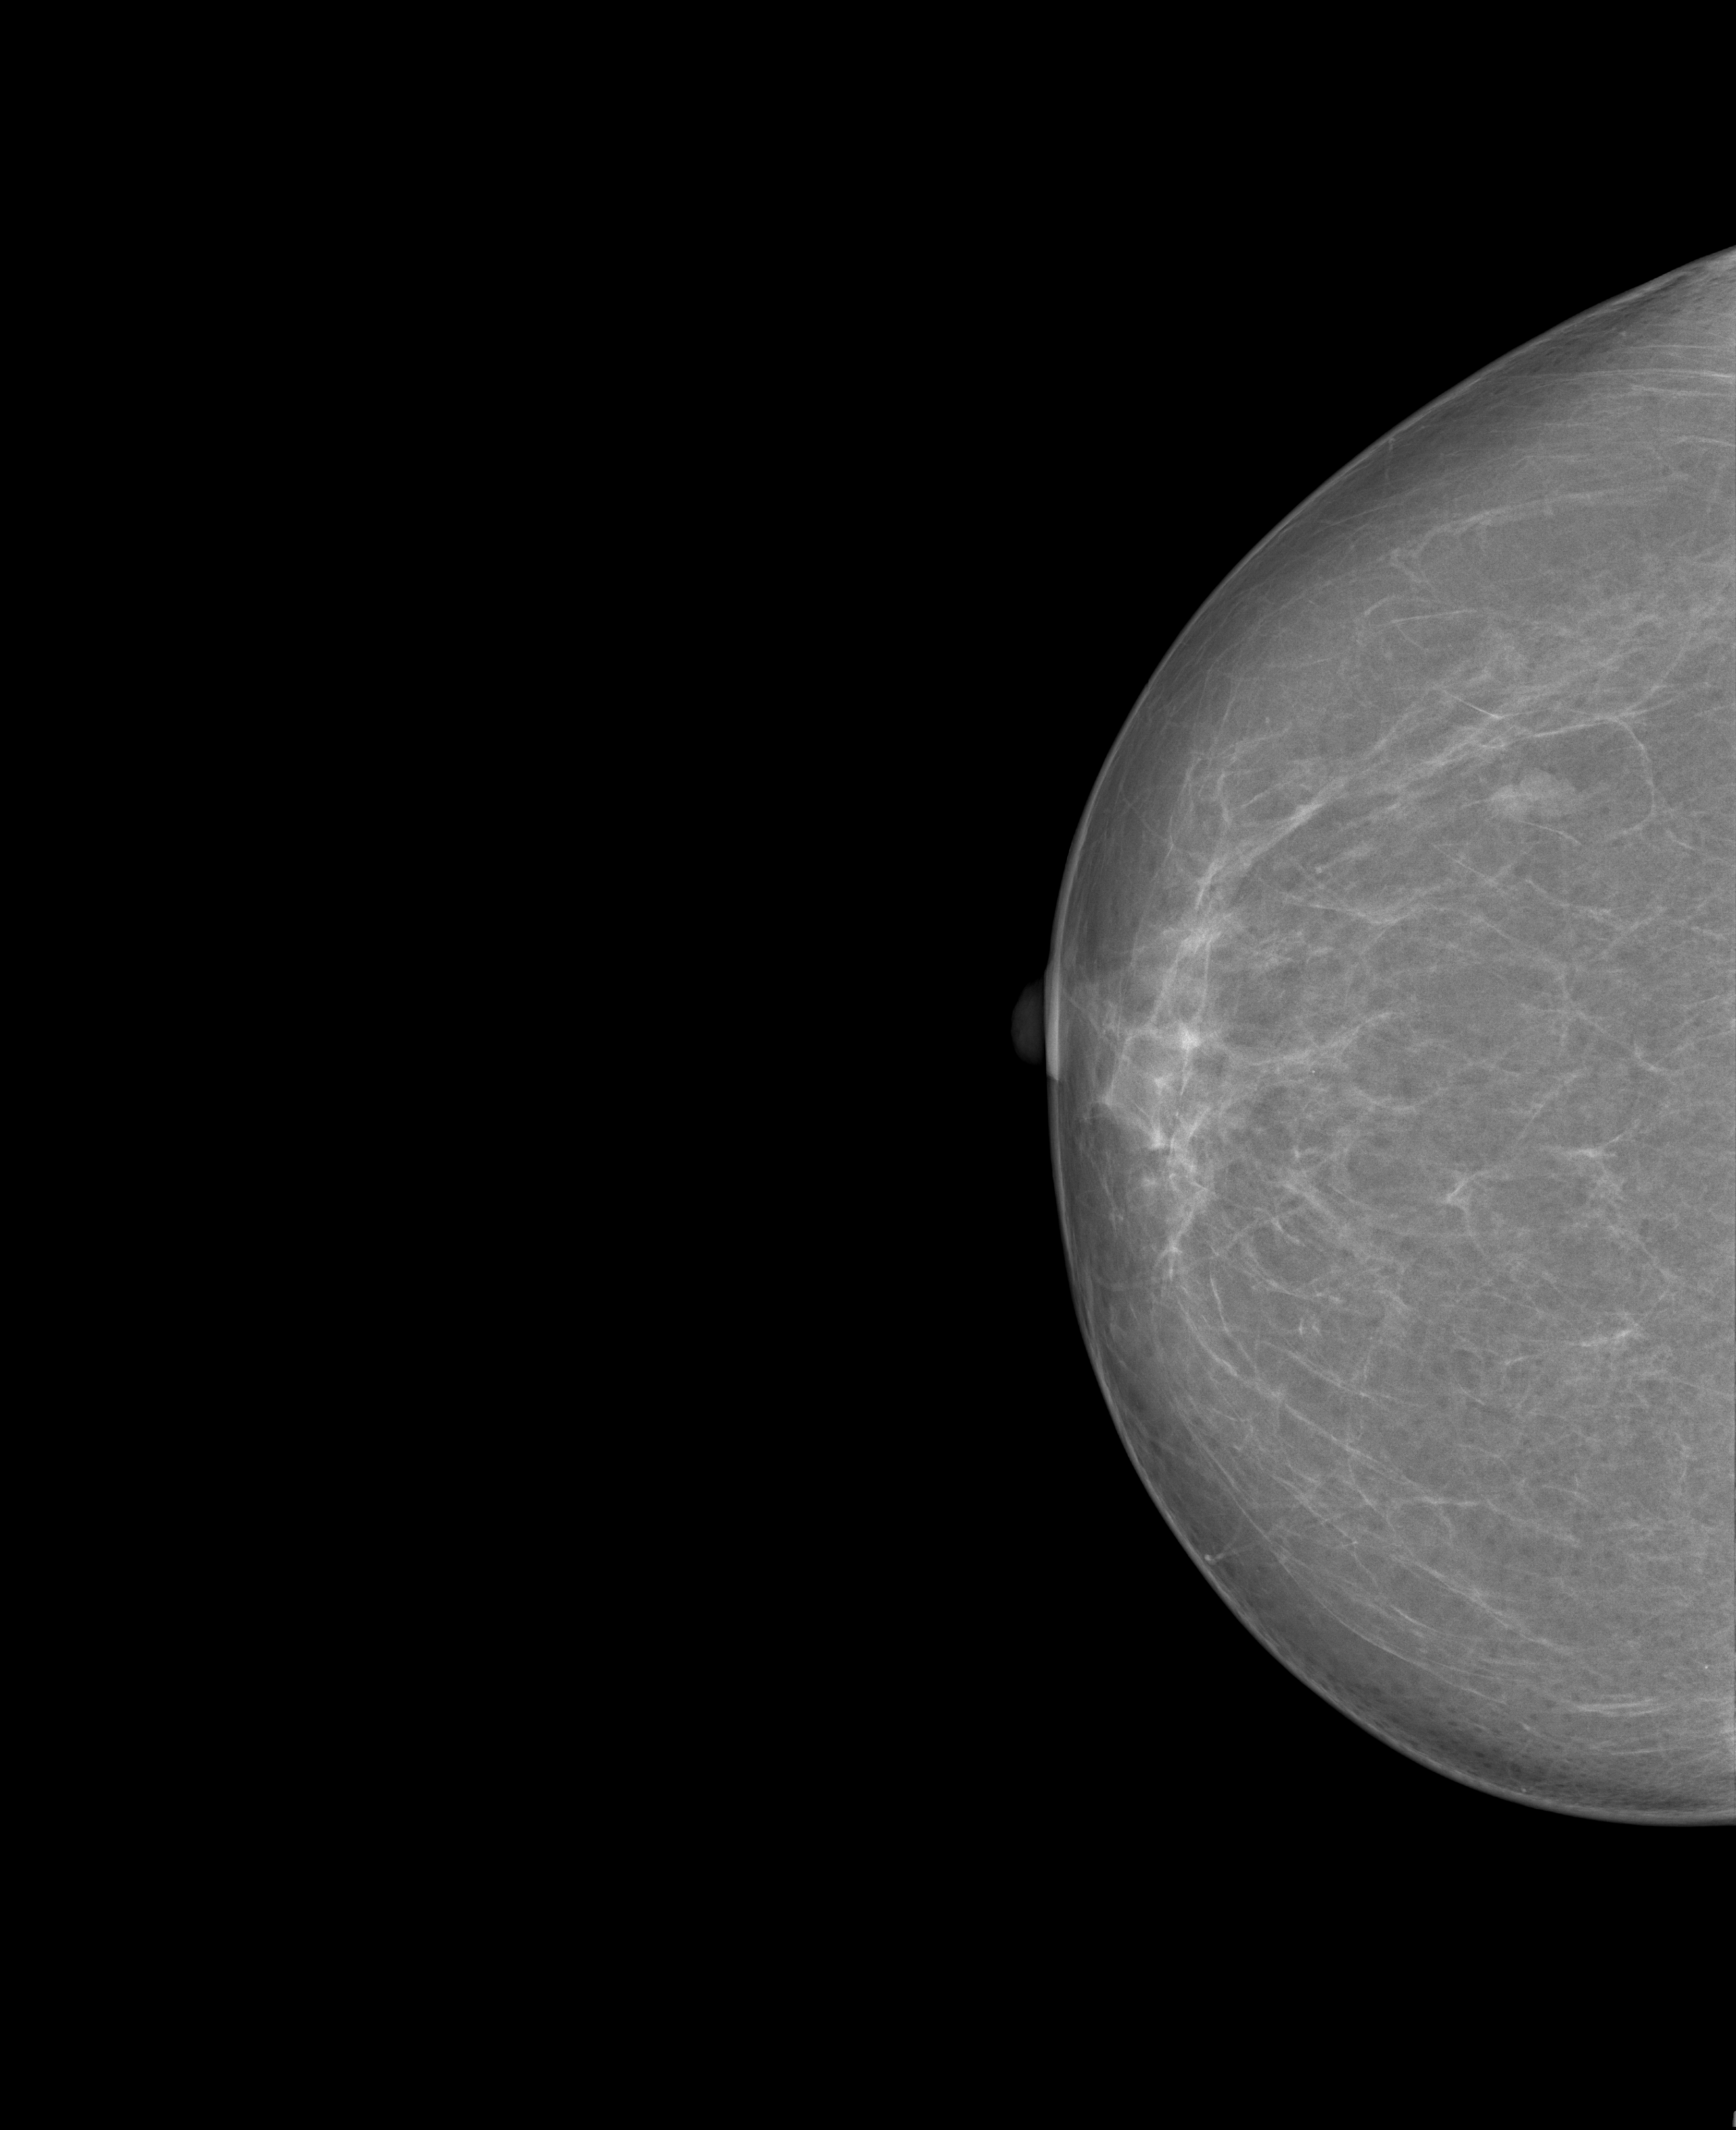
\includegraphics[height = 3.5cm]{plots/mammogram_ex2.png}
				\caption{Original}
			\end{subfigure}
			\begin{subfigure}{0.16\textwidth}
				\centering
					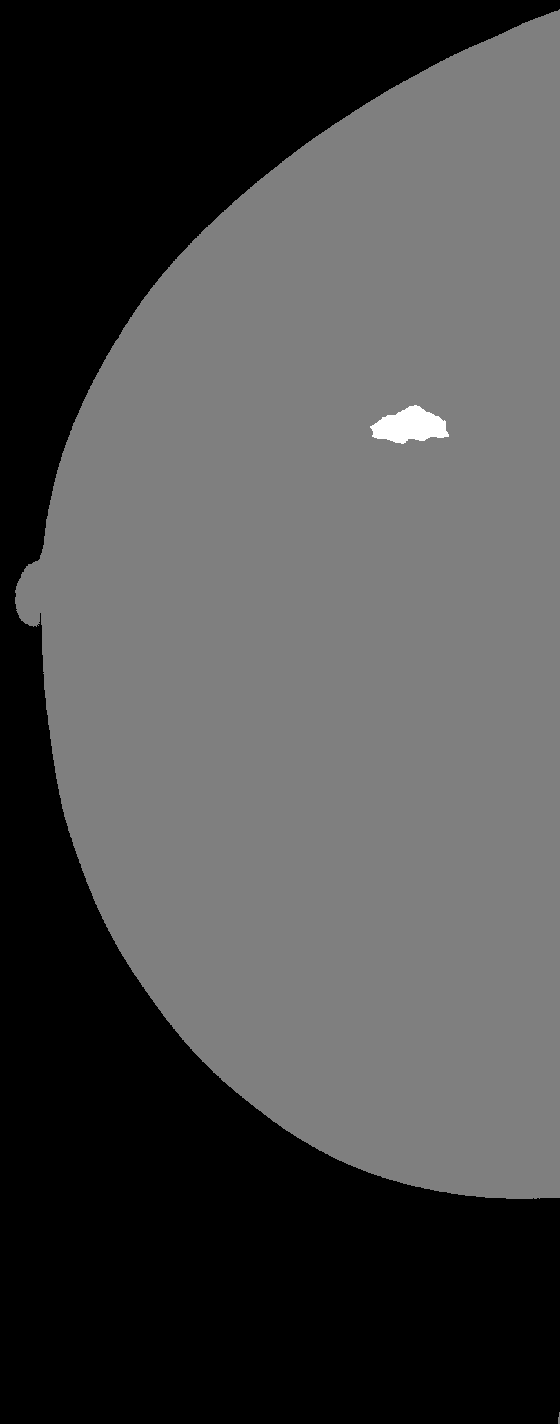
\includegraphics[height = 3.5cm]{plots/label_ex2.png}
				\caption{Label}
			\end{subfigure}
			\begin{subfigure}{0.17\textwidth}
				\centering
					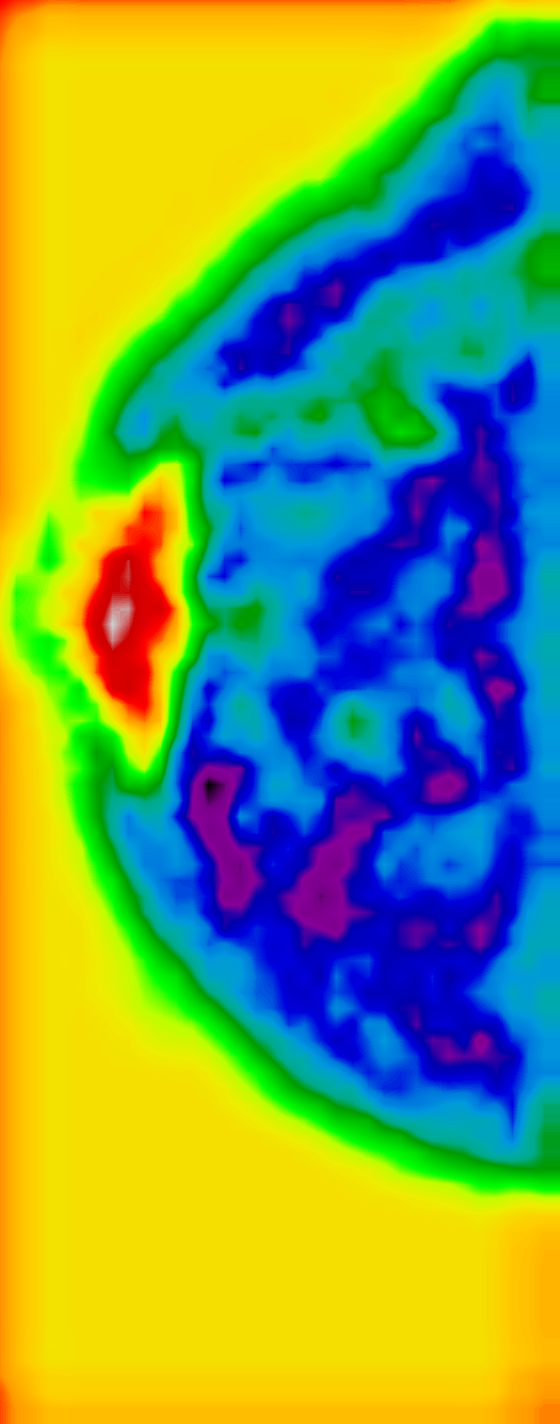
\includegraphics[height = 3.5cm]{plots/logits_ex2_v1.png}
				\caption{Prediction}
			\end{subfigure}
			\begin{subfigure}{0.22\textwidth}
				\centering
					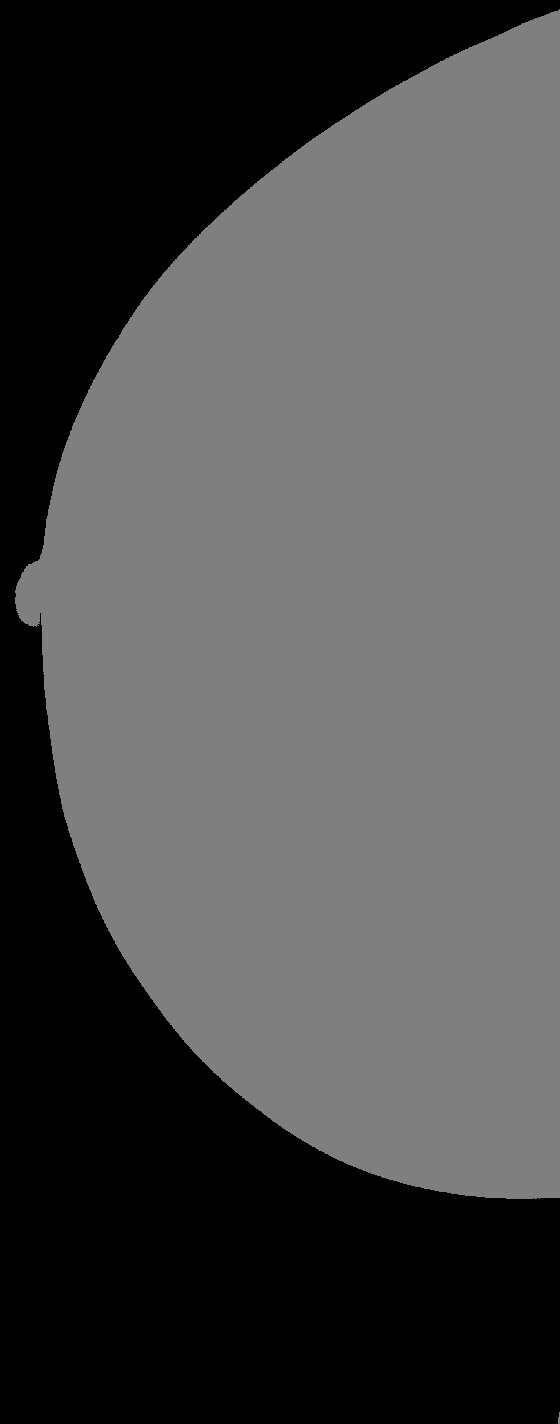
\includegraphics[height = 3.5cm]{plots/segmentation_ex2_v1.png}
				\caption{Segmentation}
			\end{subfigure}% img_108_146_1_RCC.png
		\end{figure}		
	\end{frame}
	
	\begin{frame}
		\frametitle{Experiment 2}
		To combat class imbalance, we use a loss function that weights errors over breast masses higher than errors over breast tissue. Architecture as in Experiment 1.
		
		\scriptsize
		\begin{table}[h]
			\centering
			\begin{tabular}{cccccccc}
			\hline
			\textbf{IOU}	& \textbf{F1-score}	& \textbf{G-mean} &\textbf{Accuracy}	& \textbf{Sensitivity} & \textbf{Specificity} & \textbf{Precision} & \textbf{Recall}\\
			\hline
			 0.117 & 0.21 & 0.493 & 0.981 & 0.246 & 0.989 & 0.184 & 0.246\\
			\hline
			\end{tabular}
		\end{table}
	\end{frame}
	
	\begin{frame}
		\frametitle{Qualitative results}
		\begin{figure}[h]
		\centering
			\begin{subfigure}{0.25\textwidth}
				\centering
					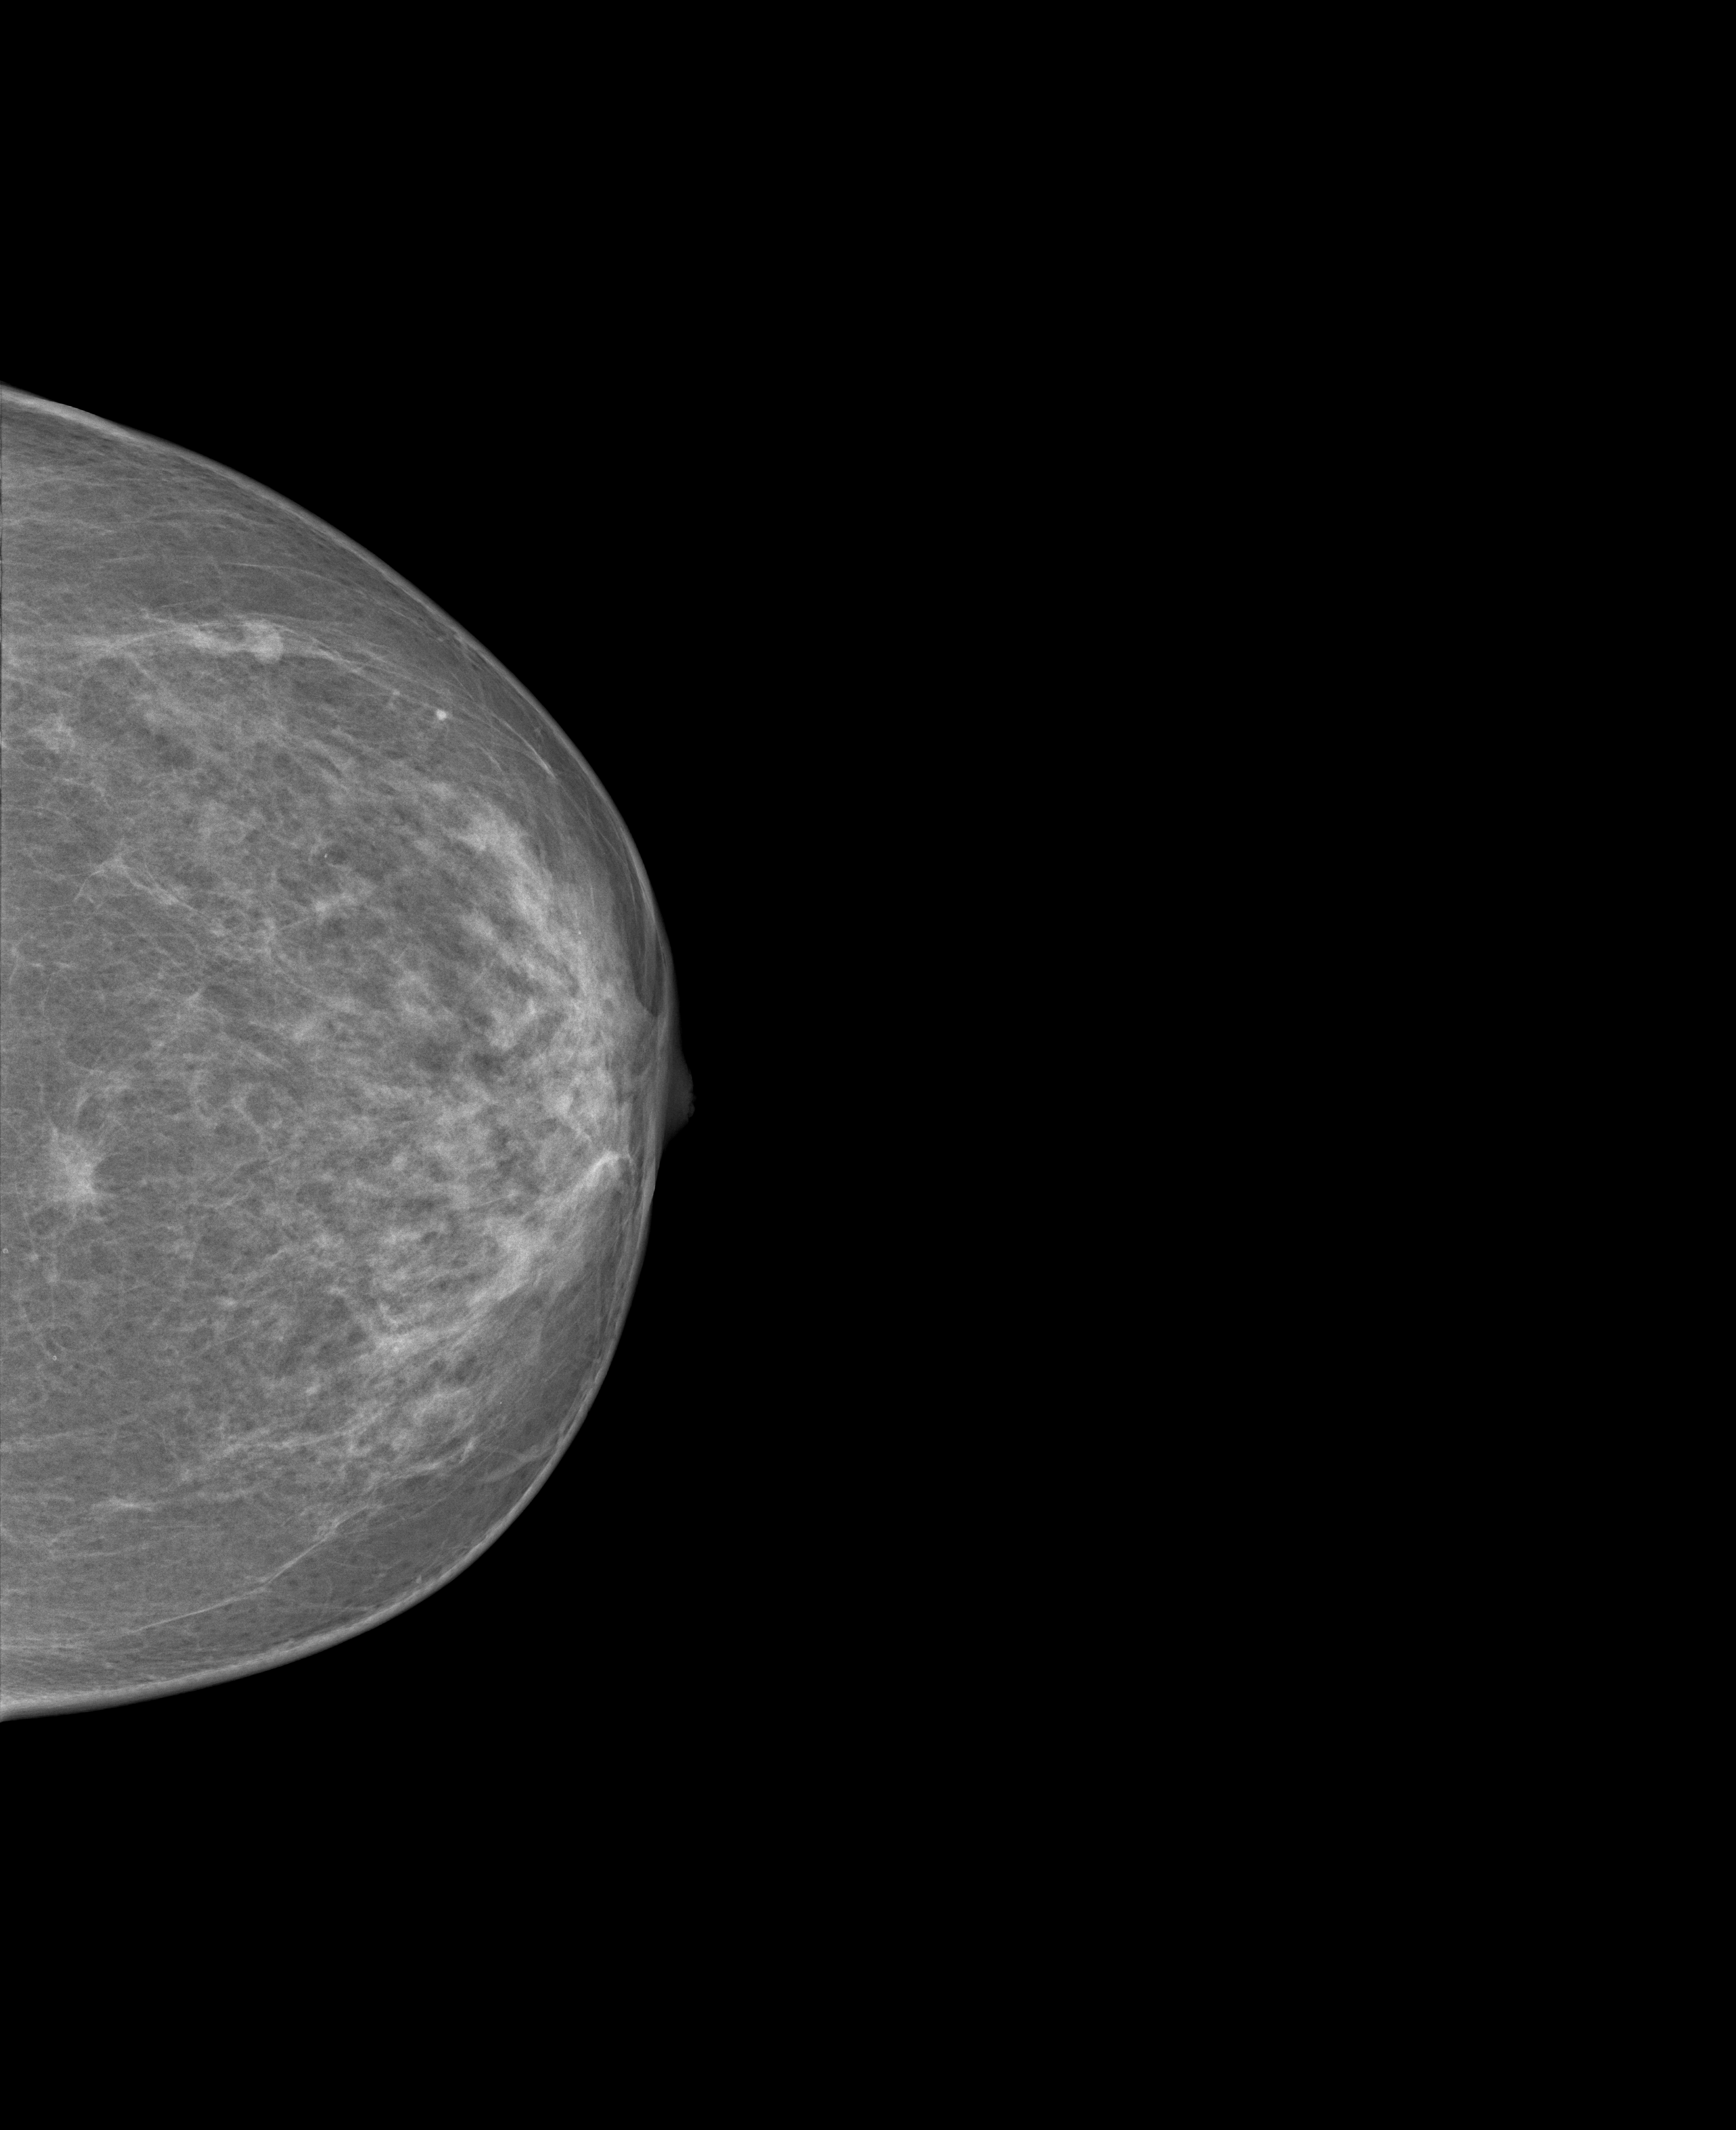
\includegraphics[height=3.5cm]{plots/mammogram_ex1.png}
			\end{subfigure}
			\begin{subfigure}{0.16\textwidth}
				\centering
					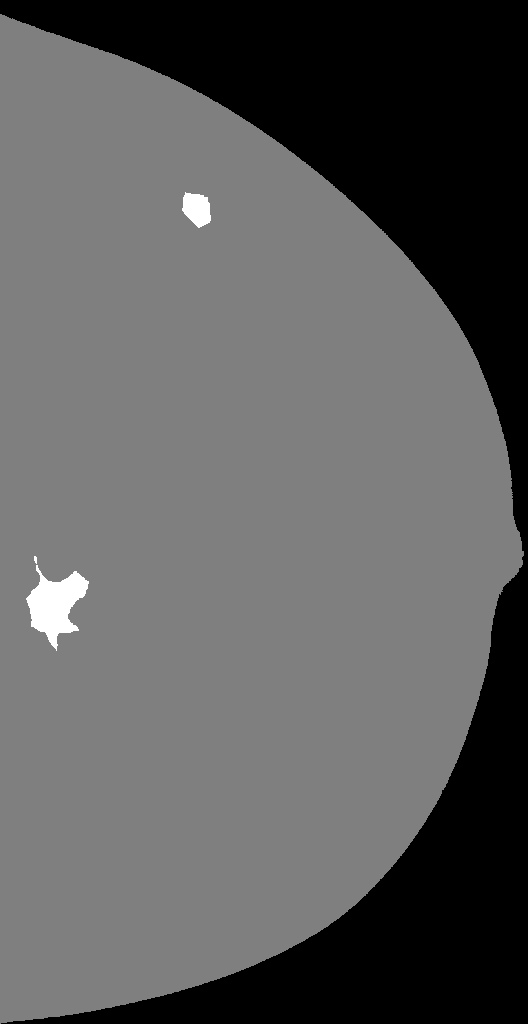
\includegraphics[height=3.5cm]{plots/label_ex1.png}
			\end{subfigure}
			\begin{subfigure}{0.17\textwidth}
				\centering
					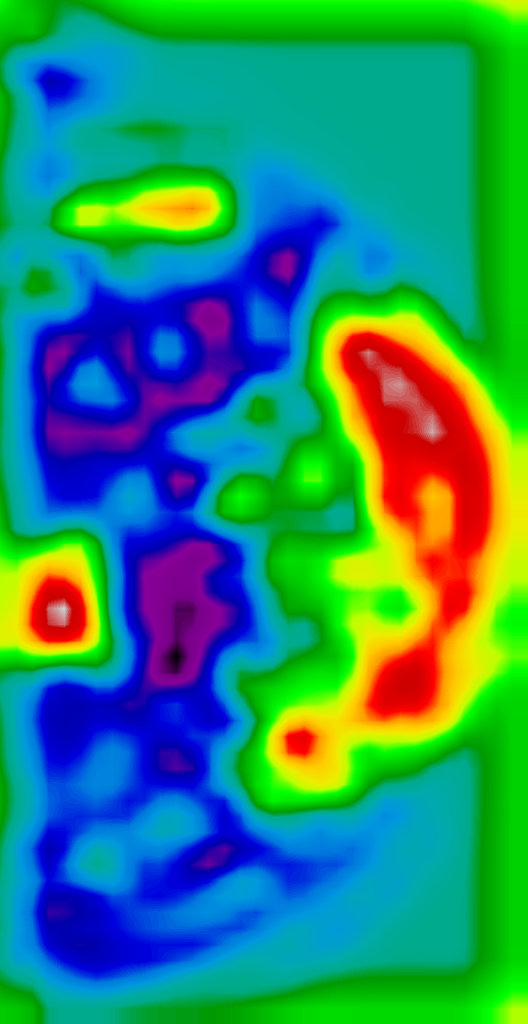
\includegraphics[height=3.5cm]{plots/logits_ex1_v2.png}
			\end{subfigure}
			\begin{subfigure}{0.22\textwidth}
				\centering
					
\includegraphics[height=3.5cm]{plots/segmentation_ex1_v2.png}
			\end{subfigure}%img_251_334_1_LCC.png
			\\
			\begin{subfigure}{0.25\textwidth}
				\centering
					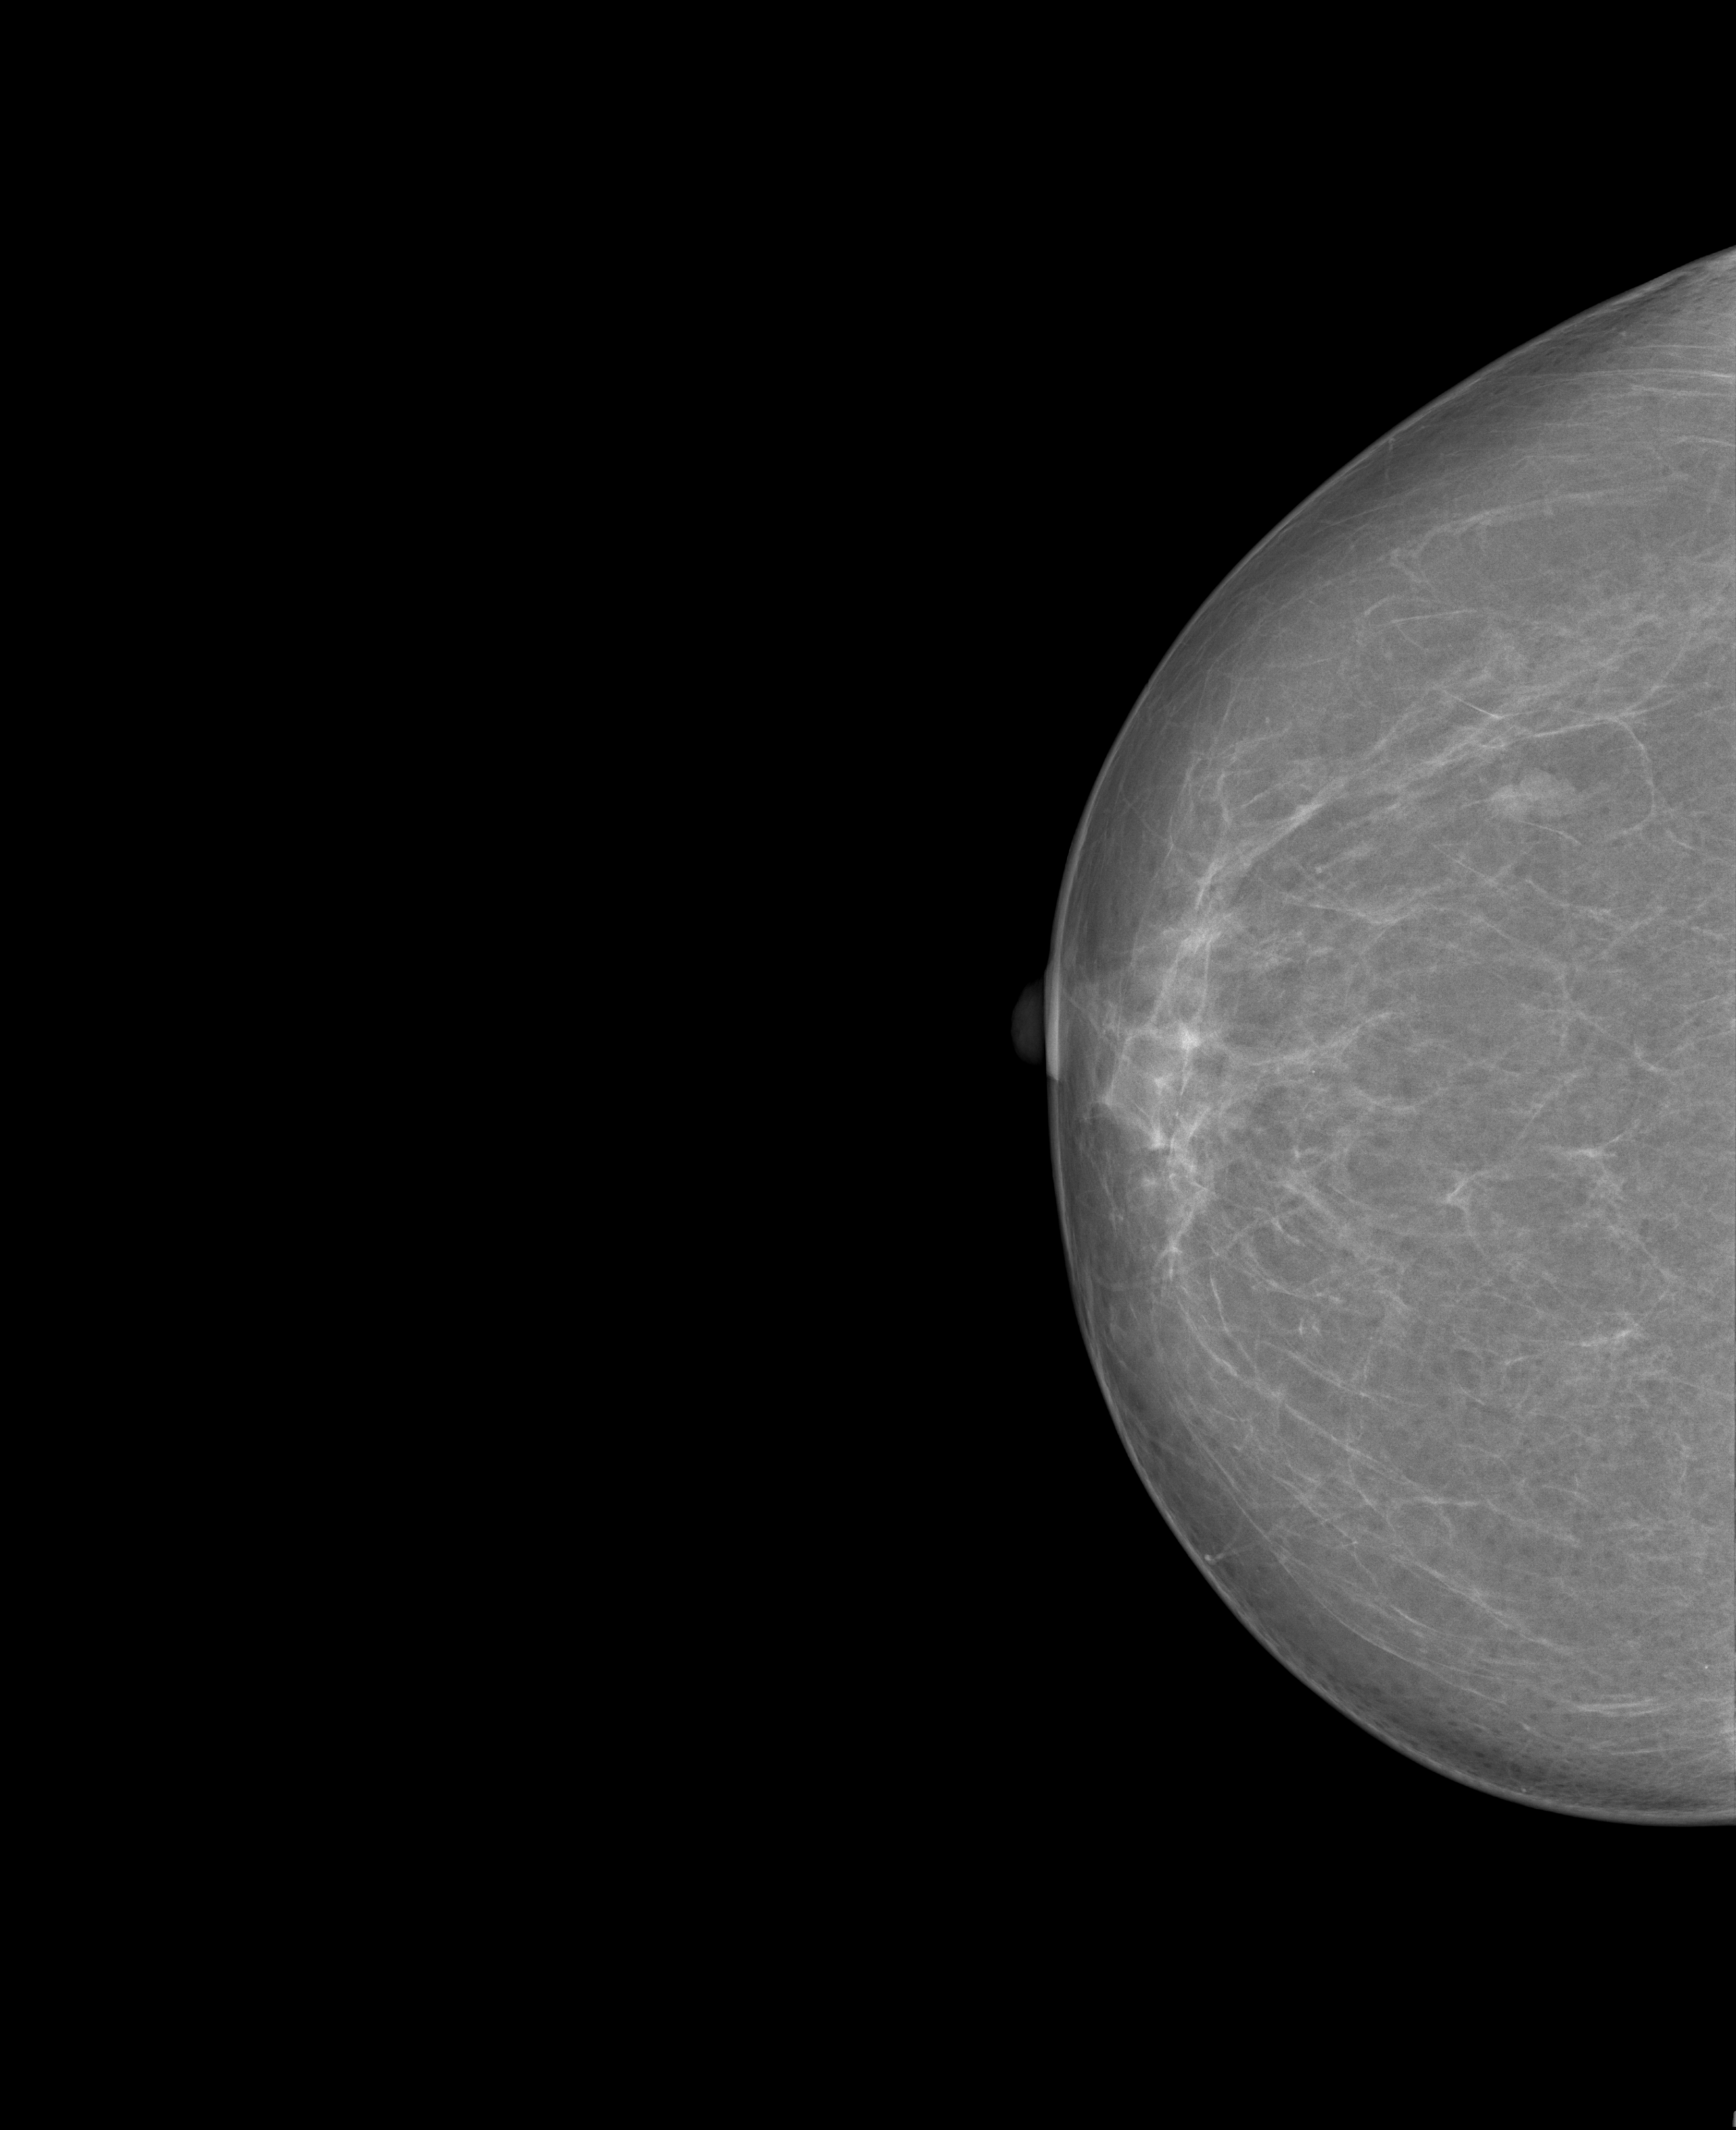
\includegraphics[height = 3.5cm]{plots/mammogram_ex2.png}
				\caption{Original}
			\end{subfigure}
			\begin{subfigure}{0.16\textwidth}
				\centering
					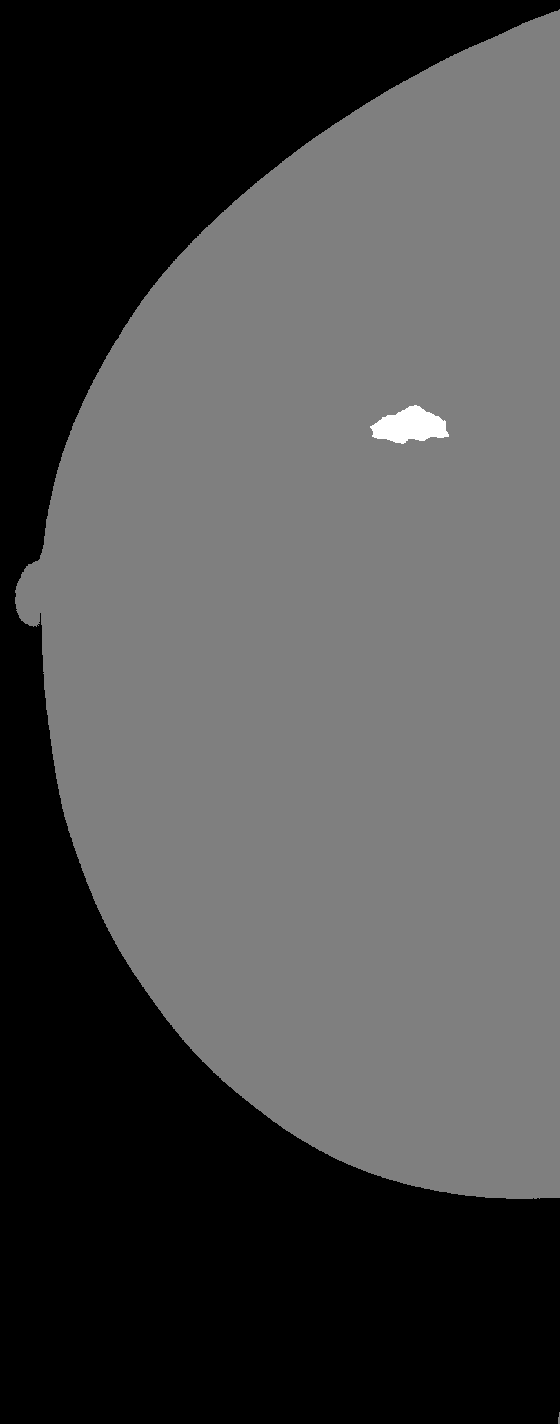
\includegraphics[height = 3.5cm]{plots/label_ex2.png}
				\caption{Label}
			\end{subfigure}
			\begin{subfigure}{0.17\textwidth}
				\centering
					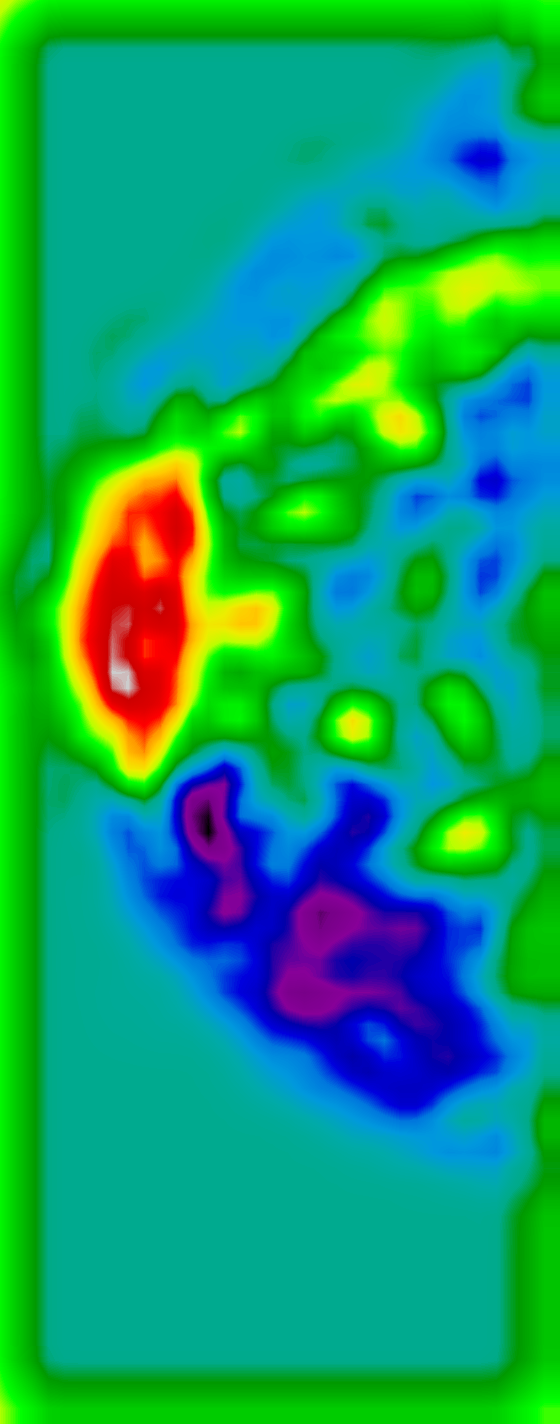
\includegraphics[height = 3.5cm]{plots/logits_ex2_v2.png}
				\caption{Prediction}
			\end{subfigure}
			\begin{subfigure}{0.22\textwidth}
				\centering
					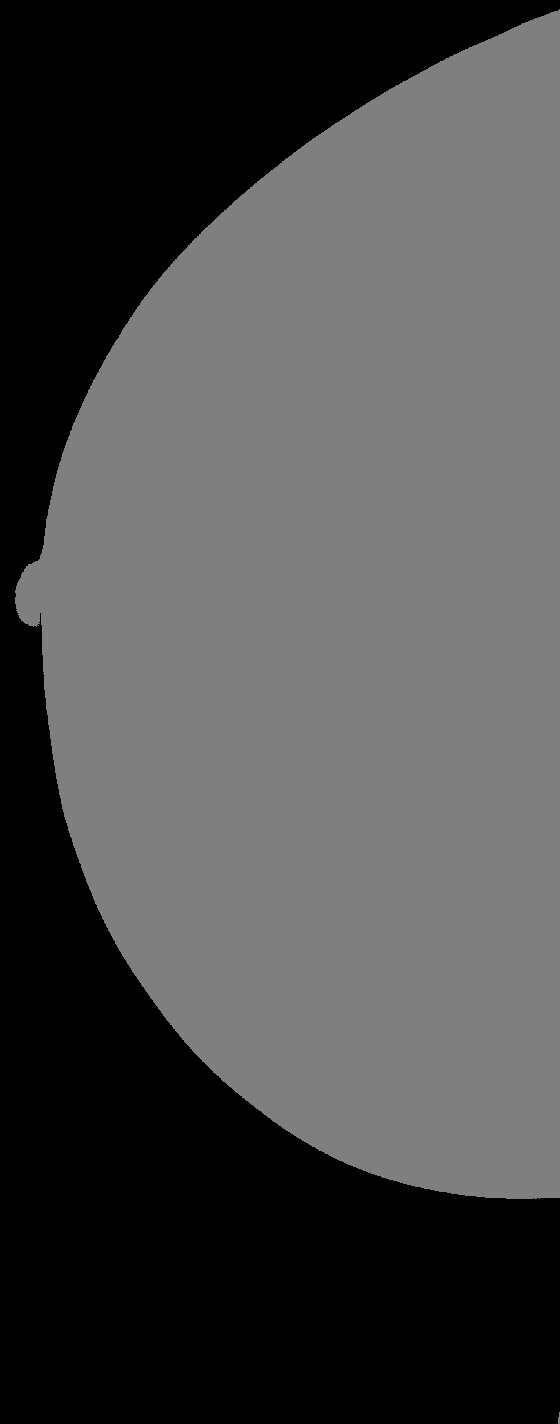
\includegraphics[height = 3.5cm]{plots/segmentation_ex2_v2.png}
				\caption{Segmentation}
			\end{subfigure}% img_108_146_1_RCC.png
		\end{figure}		
	\end{frame}
	
	\begin{frame}
		\frametitle{Experiment 3}
		Modelled on the Residual network, winner of the 2015 ImageNet. Deeper, fewer parameters and better resolution (4x).
		\footnotesize
		\begin{table}[h]
			\centering
			\begin{tabular}{lcccccr}
			\hline
			\textbf{Layer} & \textbf{Filter} & \textbf{Stride} & \textbf{Pad} & \textbf{Dilation} & \textbf{Volume} & \textbf{Parameters} \\
			\hline
			\texttt{INPUT}	&- & -	& - & - & $128 \times 128 \times 1$ & -\\
			\texttt{CONV -> LRELU}	& $6 \times 6$ & 2 & 2 & 1 & $64 \times 64 \times 32$ & 1\,184\\
			\texttt{CONV -> LRELU}	& $3 \times 3$ & 1 & 1 & 1 & $64 \times 64 \times 32$ & 9\,248\\
			\texttt{CONV -> LRELU}	& $3 \times 3$ & 2 & 1 & 1 & $32 \times 32 \times 64$ & 18\,496\\
			\texttt{CONV -> LRELU}	& $3 \times 3$ & 1 & 1 & 1 & $32 \times 32 \times 64$ & 36\,928\\
			\texttt{CONV -> LRELU}	& $3 \times 3$ & 1 & 2 & 2 & $32 \times 32 \times 128$ & 73\,856\\
			\texttt{CONV -> LRELU}	& $3 \times 3$ & 1 & 2 & 2 & $32 \times 32 \times 128$ & 147\,584\\
			\texttt{CONV -> LRELU}	& $3 \times 3$ & 1 & 2 & 2 & $32 \times 32 \times 128$ & 147\,584\\
			\texttt{CONV -> LRELU}	& $3 \times 3$ & 1 & 2 & 2 & $32 \times 32 \times 128$ & 147\,584\\
			\texttt{CONV -> LRELU}	& $3 \times 3$ & 1 & 4 & 4 & $32 \times 32 \times 256$ & 295\,168\\
			\texttt{CONV}	& $8 \times 8$ & 1 & 14 & 4 & $32 \times 32 \times 1$ & 16\,385\\
			\texttt{BILINEAR (x4)}		& - & - && - & $128 \times 128 \times 1$ & -\\
			\hline
			\end{tabular}
		\end{table}
		
		\scriptsize
		\begin{table}[h]
			\centering
			\begin{tabular}{cccccccc}
			\hline
			\textbf{IOU}	& \textbf{F1-score}	& \textbf{G-mean} &\textbf{Accuracy}	& \textbf{Sensitivity} & \textbf{Specificity} & \textbf{Precision} & \textbf{Recall}\\
			\hline
			- & - & - & - & - & - & - & -\\
			\hline
			\end{tabular}
		\end{table}
	\end{frame}
\begin{comment}
	\begin{frame}
		\frametitle{Qualitative results}
		\begin{figure}[h]
		\centering
			\begin{subfigure}{0.25\textwidth}
				\centering
					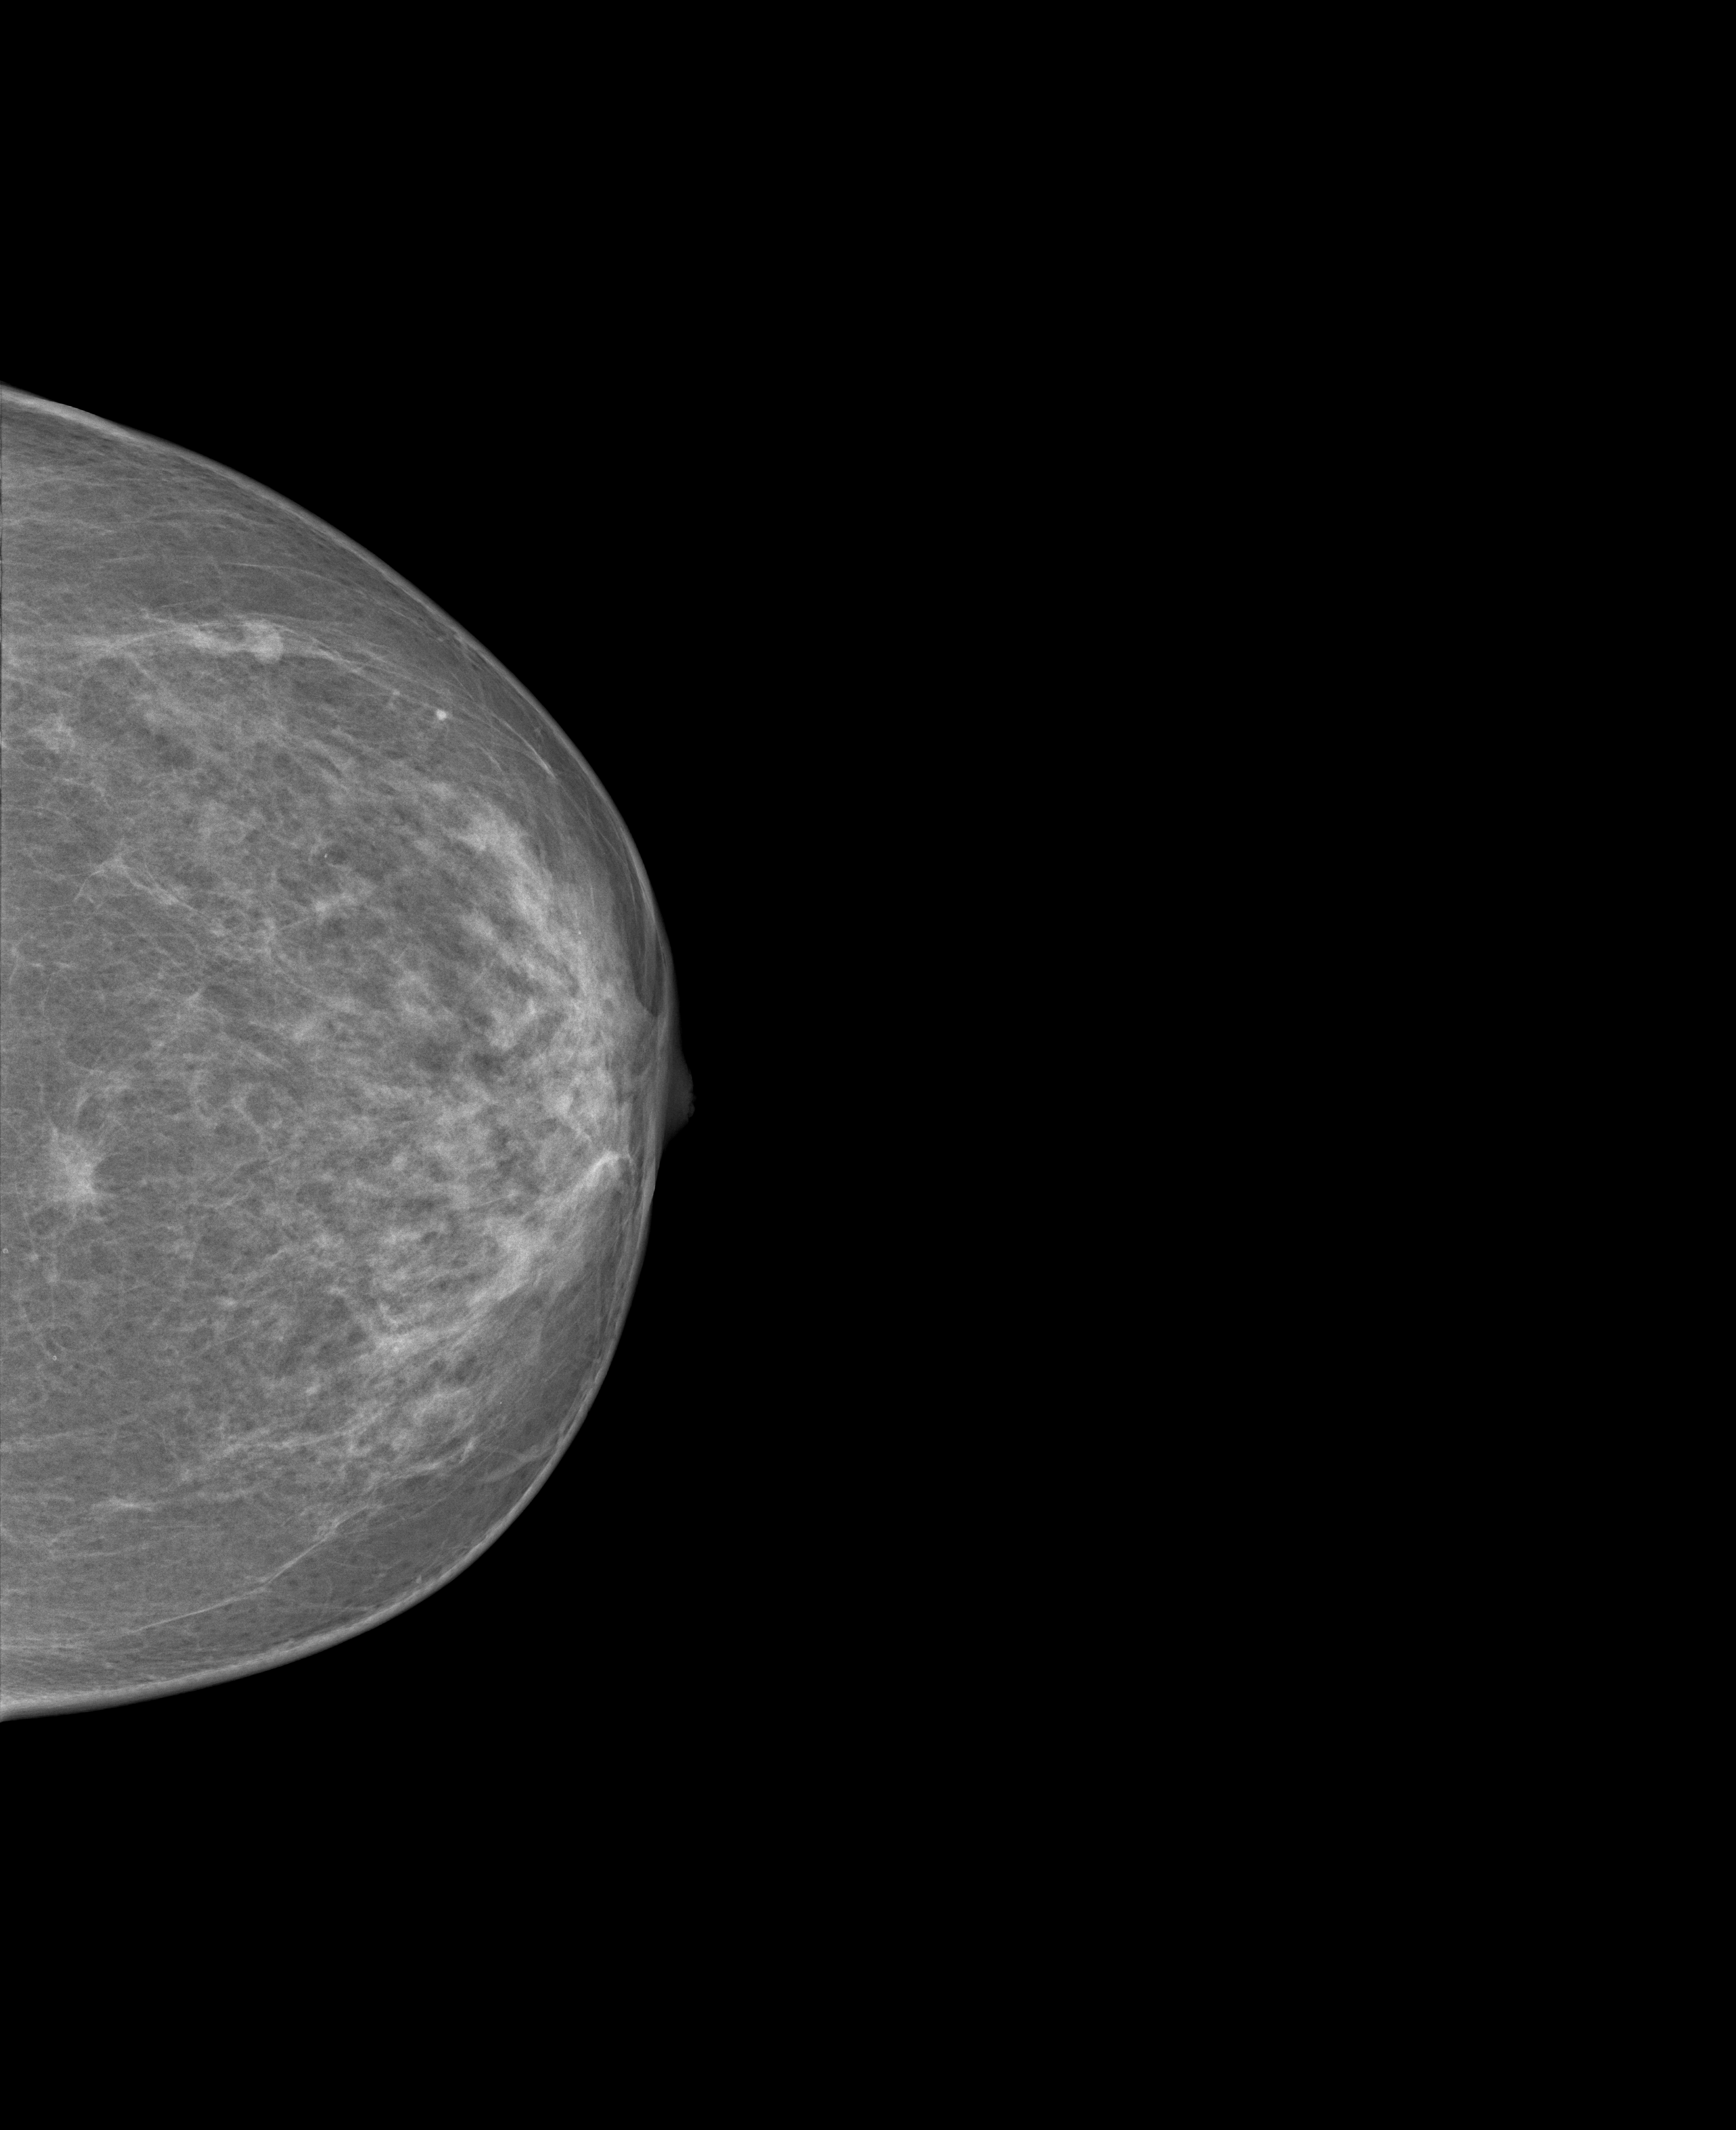
\includegraphics[height=3.5cm]{plots/mammogram_ex1.png}
			\end{subfigure}
			\begin{subfigure}{0.16\textwidth}
				\centering
					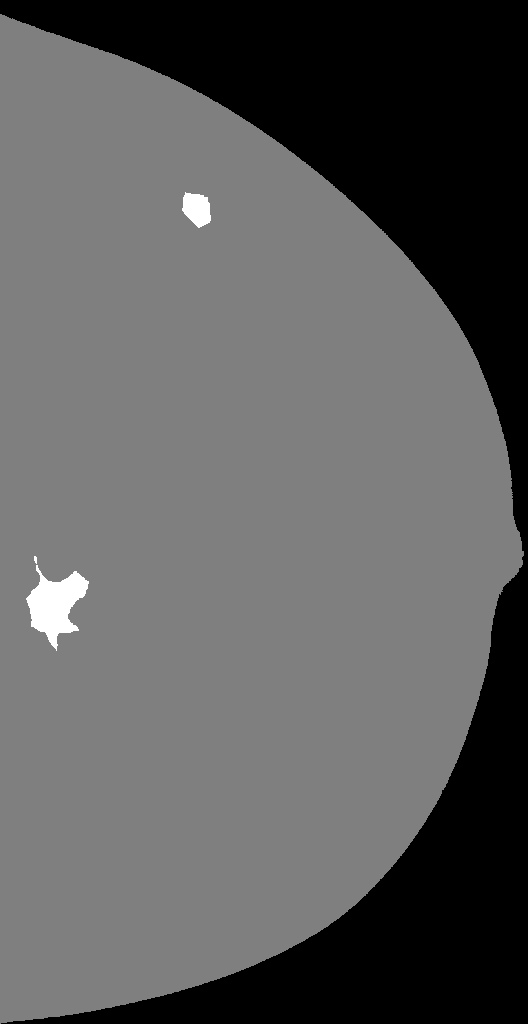
\includegraphics[height=3.5cm]{plots/label_ex1.png}
			\end{subfigure}
			\begin{subfigure}{0.17\textwidth}
				\centering
					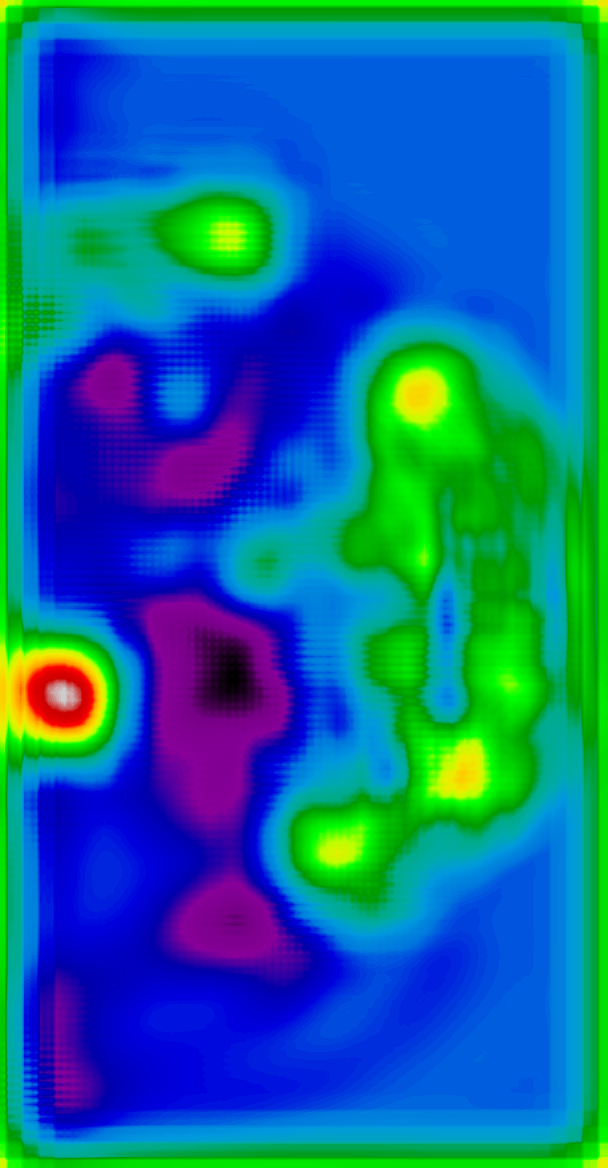
\includegraphics[height=3.5cm]{plots/logits_ex1_v3.png}
			\end{subfigure}
			\begin{subfigure}{0.22\textwidth}
				\centering
					
\includegraphics[height=3.5cm]{plots/segmentation_ex1_v3.png}
			\end{subfigure}% img_108_146_1_RCC.png
			\\
			\begin{subfigure}{0.25\textwidth}
				\centering
					\includegraphics[height = 3.5cm]{plots/mammogram_ex2.png}
				\caption{Original}
			\end{subfigure}
			\begin{subfigure}{0.16\textwidth}
				\centering
					\includegraphics[height = 3.5cm]{plots/label_ex2.png}
				\caption{Label}
			\end{subfigure}
			\begin{subfigure}{0.17\textwidth}
				\centering
					\includegraphics[height = 3.5cm]{plots/logits_ex2_v3.png}
				\caption{Prediction}
			\end{subfigure}
			\begin{subfigure}{0.22\textwidth}
				\centering
					\includegraphics[height = 3.5cm]{plots/segmentation_ex2_v3.png}
				\caption{Segmentation}
			\end{subfigure}%img_251_334_1_LCC.png
		\end{figure}		
	\end{frame}
\end{comment}
	\begin{frame}
		\frametitle{Writing the thesis}
		65 pages and counting...
	\end{frame}
	
	
	\section[Conclusion]{Conclusion}
	\begin{frame}
		\frametitle{Future work}
		\begin{itemize}
			\item Train networks with increasing number of examples
			\item Train simpler network with all data
			\item Write thesis
		\end{itemize}
	\end{frame}

	\begin{frame}[c]
		\begin{center}
			\begin{figure}
				\includegraphics[width=0.25\textwidth]{plots/questions.png}
			\end{figure}
		\end{center}
	\end{frame}

\end{document}
